\documentclass[12pt, a4paper]{article}

% ── Paquetes ──────────────────────────────────────────────────
\usepackage[utf8]{inputenc}
\usepackage[T1]{fontenc}
\usepackage[spanish,es-noshorthands]{babel}
\usepackage{amsmath, amssymb, amsthm}
\usepackage{graphicx}
\usepackage{booktabs}
\usepackage[round,authoryear]{natbib}
\usepackage{hyperref}
\usepackage{geometry}
\usepackage{setspace}
\usepackage{lineno}
\usepackage{xcolor}
\usepackage{caption}
\usepackage{subcaption}
\usepackage{float}
\usepackage{siunitx}

\geometry{margin=2.5cm}
\doublespacing
\linenumbers

\sisetup{output-decimal-marker={,}, group-separator={\,}}

\hypersetup{
  colorlinks = true,
  linkcolor  = blue,
  citecolor  = blue,
  urlcolor   = blue
}

% ── Información del manuscrito ────────────────────────────────
\title{Análisis espacial de la susceptibilidad a los movimientos en masa en el
       Valle de Aburrá (Colombia) mediante un Proceso de Cox Log-Gaussiano
       con aproximación SPDE-INLA}

\author{
  Edier Aristizábal\textsuperscript{1,*}\\[6pt]
  \small\textsuperscript{1} Universidad Nacional de Colombia, Sede Medellín,
  Departamento de Geociencias y Medio Ambiente\\
  \small\textsuperscript{*} Autor para correspondencia:
  \href{mailto:evaristizabalg@unal.edu.co}{evaristizabalg@unal.edu.co}
}

\date{\today}

% ─────────────────────────────────────────────────────────────
\begin{document}
\maketitle

\begin{abstract}
Los movimientos en masa representan una de las amenazas naturales más destructivas
en las regiones montañosas tropicales, ocasionando pérdidas humanas y económicas
significativas en cuencas densamente urbanizadas como el Valle de Aburrá, Colombia.
La modelación estadística de la susceptibilidad a este tipo de fenómenos ha recurrido
históricamente a la regresión logística o a clasificadores de aprendizaje automático
que tratan el inventario como una respuesta binaria de presencia-ausencia, ignorando
la estructura espacial propia de los datos de proceso puntual. Este estudio propone
un marco de modelación mediante el Proceso de Cox Log-Gaussiano (LGCP) que modela
explícitamente la intensidad espacialmente variable de la ocurrencia de movimientos
en masa. La inferencia bayesiana se realiza con la Aproximación de Laplace Anidada
Integrada (INLA) combinada con la aproximación por Ecuación Diferencial Parcial
Estocástica (SPDE) del campo aleatorio gaussiano latente (GRF), garantizando un
cómputo eficiente en dominios espaciales extensos. La intensidad
$\lambda(\mathbf{s})$ se descompone en una componente determinística impulsada
por predictores topográficos ---pendiente, Índice Topográfico de Humedad (TWI) y
aspecto--- y una componente aleatoria espacialmente estructurada que captura el
agrupamiento residual no explicado. El modelo se ajusta a un inventario de
\num{2504} movimientos en masa sobre un dominio de \SI{353,7}{km^2}. La pendiente
($\hat{\beta}_1 = 13{,}09$, IC\,95\%: $[12{,}69,\;13{,}48]$) y el TWI
($\hat{\beta}_2 = 13{,}00$, IC\,95\%: $[12{,}64,\;13{,}37]$) son los principales
impulsores positivos de la intensidad, reflejando el papel mecánico de la gravedad
y la concentración de presión de poros en la inestabilidad de laderas. El aspecto
muestra un efecto positivo más débil pero significativo ($\hat{\beta}_3 = 5{,}70$,
IC\,95\%: $[5{,}50,\;5{,}90]$). El GRF latente presenta un rango de correlación
de $\hat{\rho} = 5{,}01$ km y una varianza marginal de $\hat{\sigma}^2 = 2{,}62$,
evidenciando agrupamiento espacial residual atribuible a factores geológicos,
pedológicos y antrópicos no incluidos. El AUC del modelo es $0{,}651$. El marco
propuesto ofrece una base probabilística rigurosa para la evaluación de la amenaza
y constituye una extensión natural hacia la modelación espacio-temporal cuando se
dispone de fechas de ocurrencia.

\smallskip
\noindent\textbf{Palabras clave:} susceptibilidad a movimientos en masa; Proceso
de Cox Log-Gaussiano; SPDE-INLA; proceso puntual espacial; Valle de Aburrá;
inferencia bayesiana; campo aleatorio gaussiano; Índice Topográfico de Humedad.
\end{abstract}

% ─────────────────────────────────────────────────────────────
\section{Introducción}
\label{sec:intro}
% ─────────────────────────────────────────────────────────────

Los movimientos en masa constituyen una de las amenazas naturales más frecuentes
y dañinas en los trópicos andinos, donde la combinación de topografía escarpada,
precipitaciones convectivas intensas y rápida expansión urbana genera condiciones
de alta susceptibilidad \citep{reichenbach2018}. El Valle de Aburrá, un estrecho
valle interandino en el noroccidente de Colombia que alberga el Área Metropolitana
de Medellín (aproximadamente 3,9 millones de habitantes), ha experimentado
recurrentes eventos de movimiento en masa que han ocasionado pérdidas significativas
de vidas humanas e infraestructura \citep{aristizabal2016, parra2019}. La
disponibilidad de modelos espacialmente explícitos de susceptibilidad es, por
tanto, una necesidad imperiosa para la reducción del riesgo, la planificación
territorial y el diseño de sistemas de alerta temprana.

La modelación estadística de la susceptibilidad a los movimientos en masa tiene
una larga historia basada en la regresión logística \citep{reichenbach2018}.
La mayor parte de los enfoques proyectan el inventario sobre una cuadrícula
regular, asignan etiquetas binarias de presencia-ausencia a las celdas y modelan
la probabilidad de ocurrencia en función de atributos del terreno como la pendiente,
la curvatura, la litología y la cobertura del suelo \citep{guzzetti2005, lombardo2018}.
Aunque operativamente conveniente, esta discretización acarrea una pérdida de
información espacial y trata implícitamente todas las áreas sin eventos registrados
como ``ausencia'', confundiendo la ausencia verdadera con la falta de observación.
Además, la asignación de seudoausencias introduce subjetividad y puede alterar
los estimados de los coeficientes cuando la proporción de presencias es alta
\citep{lombardo2018}.

Un marco más riguroso para el análisis de catálogos de eventos georeferenciados
es el Proceso Puntual Espacial. En este paradigma, el inventario de movimientos
en masa se trata como una realización de un conjunto aleatorio de puntos en el
dominio de estudio $\Omega \subset \mathbb{R}^2$, y la inferencia estadística
apunta a la función de intensidad espacialmente variable $\lambda(\mathbf{s})$
que gobierna el número esperado de eventos por unidad de área en la localización
$\mathbf{s}$ \citep{diggle2013}. Esta función de intensidad tiene una interpretación
física directa: es proporcional a la probabilidad de que se inicie un movimiento
en masa en cualquier punto del terreno, dada la configuración topográfica,
geológica e hidrológica local. El Proceso de Cox Log-Gaussiano
\citep[LGCP;][]{moller1998} es un miembro especialmente flexible de esta familia:
la log-intensidad se modela como un campo aleatorio gaussiano (GRF), que acomoda
naturalmente tanto tendencias suaves impulsadas por covariables ambientales como
agrupamiento espacial residual derivado de factores no observados o no medibles,
como la variabilidad litológica y la heterogeneidad del uso del suelo.

A pesar de su atractivo teórico, la aplicación práctica del LGCP ha sido limitada
por la carga computacional de la inferencia sobre GRF, que en la implementación
ingenua escala como $\mathcal{O}(n^3)$ con el número de observaciones.
\citet{lindgren2011} resolvieron este cuello de botella demostrando que un GRF
con covarianza de Matérn puede representarse como la solución de una Ecuación
Diferencial Parcial Estocástica (SPDE) sobre una triangulación de Delaunay,
cuya discretización produce un Campo Markoviano Gaussiano Aleatorio (GMRF) disperso.
La inferencia sobre GMRFs es tratable mediante la Aproximación de Laplace Anidada
Integrada \citep[INLA;][]{rue2009, rue2017}, que computa marginales posteriores
sin muestreo de Monte Carlo por cadenas de Markov, reduciendo el tiempo de cómputo
en órdenes de magnitud. El paquete \texttt{inlabru} \citep{bachl2019} integra
este marco en una interfaz de alto nivel para modelos de proceso puntual.

La aplicación del LGCP-SPDE-INLA a los movimientos en masa sigue siendo escasa
en la literatura. \citet{lombardo2019} demostraron el enfoque para flujos de
detritos en Sicilia, y \citet{lombardo2020} lo extendieron a contextos
espacio-temporales. En ambos estudios, el marco de proceso puntual superó a los
enfoques de regresión logística en términos de consistencia probabilística y
capacidad de cuantificar la incertidumbre espacial. Sin embargo, ningún estudio
previo ha aplicado este marco en los Andes tropicales, donde la heterogeneidad
geológica, la intensidad de los regímenes de precipitación y la presión del
crecimiento urbano sobre las laderas crean un entorno de modelación particularmente
complejo.

Los objetivos de este estudio son: (i) especificar y ajustar un modelo
LGCP-SPDE-INLA para los movimientos en masa en el Valle de Aburrá; (ii) cuantificar
los efectos marginales de los predictores topográficos sobre la intensidad de
ocurrencia; (iii) cartografiar la superficie de intensidad posterior y su
incertidumbre espacial; y (iv) evaluar el desempeño discriminativo del modelo
mediante el Área Bajo la Curva ROC (AUC) y diagnósticos complementarios.

% ─────────────────────────────────────────────────────────────
\section{Área de estudio y datos}
\label{sec:data}
% ─────────────────────────────────────────────────────────────

\subsection{Área de estudio}

El Valle de Aburrá es un valle de aproximadamente \SI{1165}{km^2} situado en la
Cordillera Central de los Andes colombianos ($6°6'$--$6°41'$N, $75°45'$--$75°21'$O).
Las elevaciones oscilan entre aproximadamente 1300 m s.n.m. en el fondo del valle
y más de 3200 m s.n.m. en las crestas adyacentes; las pendientes superan
frecuentemente los $35°$ en los flancos del valle. El clima es tropical bimodal,
con precipitaciones medias anuales de 1500 a 2500 mm distribuidas en dos temporadas
lluviosas (marzo-mayo y septiembre-noviembre). El sustrato geológico consiste
predominantemente en gneis, esquistos y anfibolitas del Complejo Cajamarca,
cubiertos localmente por regolito grueso y coluviones cuaternarios susceptibles
a fallas translacionales superficiales y flujos de detritos. La alta densidad
poblacional (más de 3,9 millones de habitantes) hace que la exposición a los
movimientos en masa sea excepcionalmente alta, con numerosos sectores residenciales
construidos sobre laderas inestables.

El dominio de estudio $\Omega$ se definió como la intersección del casco convexo
del inventario de movimientos en masa (ampliado con un buffer de \SI{500}{m})
y el área cubierta por el modelo digital de elevación, obteniendo un área efectiva
de \SI{353,67}{km^2}.

\subsection{Inventario de movimientos en masa}

El inventario utilizado comprende \num{2504} eventos de movimiento en masa
(deslizamientos superficiales, flujos de detritos y deslizamientos translacionales)
recopilados a partir de registros históricos, interpretación de fotografías aéreas
y levantamientos de campo. Los eventos están georeferenciados como localizaciones
puntuales que representan la zona de iniciación de cada movimiento, proyectados
en el sistema de referencia MAGNA-SIRGAS (EPSG:9377). La densidad espacial media
es de aproximadamente 7,08 eventos km$^{-2}$ sobre el dominio de estudio, con
agrupamiento pronunciado a lo largo de los flancos escarpados del valle del
río Medellín y sus tributarios, especialmente en zonas de convergencia topográfica
donde la acumulación de flujo y las presiones de poros son más elevadas
(Figura~\ref{fig:inventario}). La distribución espacial del inventario revela
que los movimientos en masa no son aleatorios en el espacio: se concentran
preferentemente en laderas con pendientes superiores a $25°$ y en proximidad a
quebradas, indicando un control topohidrológico dominante sobre la iniciación.

\begin{figure}[H]
  \centering
  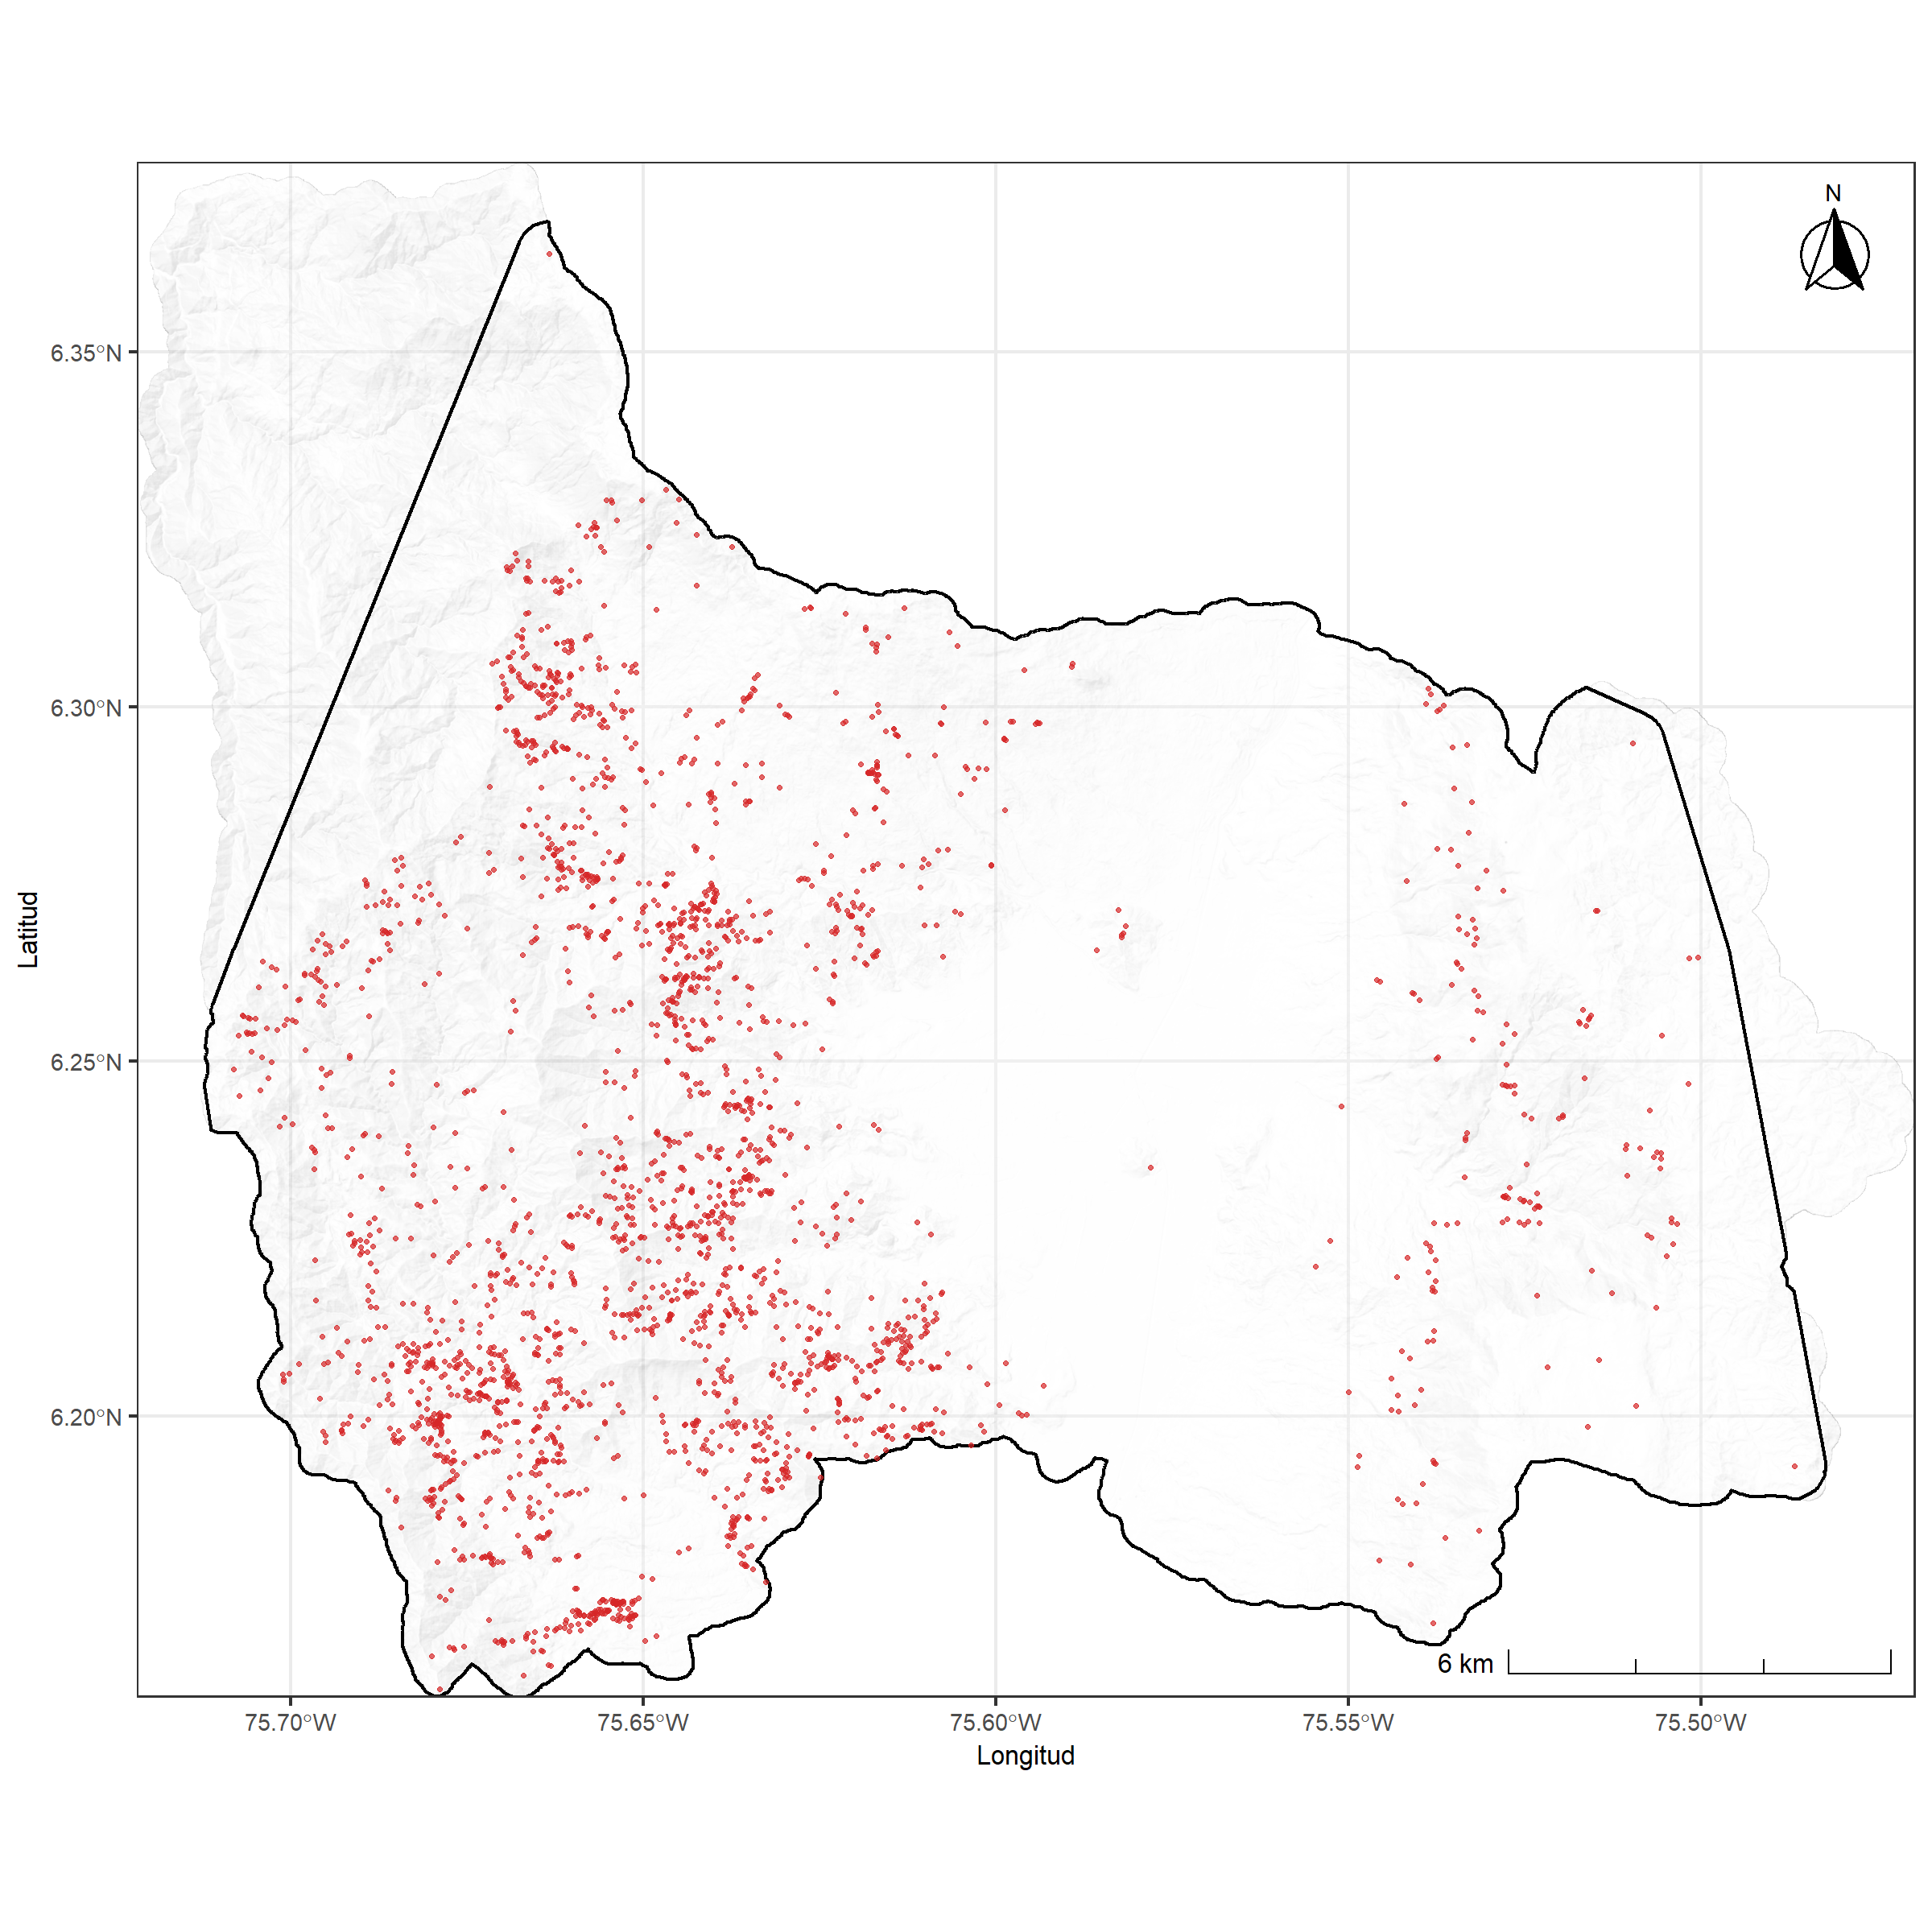
\includegraphics[width=0.75\linewidth]{FIG/00_inventario_deslizamientos.png}
  \caption{Localización espacial de los \num{2504} movimientos en masa registrados
           en el dominio de estudio del Valle de Aburrá. Cada punto rojo representa
           la zona de iniciación de un evento. El hillshade multidireccional del
           modelo digital de elevación permite apreciar la complejidad del relieve
           del valle interandino. El agrupamiento a lo largo de los flancos del
           valle y las quebradas es evidente. El contorno negro delimita el dominio
           de estudio $\Omega$ de \SI{353,67}{km^2}. Sistema de referencia:
           MAGNA-SIRGAS (EPSG:9377); coordenadas geográficas WGS84.}
  \label{fig:inventario}
\end{figure}

\subsection{Covariables topográficas}

Tres covariables topográficas se derivaron de un MDE de \SI{10}{m} de resolución
obtenido a partir de imágenes de radar de apertura sintética procesadas en el
sistema de referencia MAGNA-SIRGAS (Tabla~\ref{tab:covstats}):

\begin{enumerate}
  \item \textbf{Pendiente} ($\beta$, grados): calculada como la derivada de primer
  orden del MDE. Es el factor mecánico primario en la iniciación de deslizamientos
  superficiales: bajo el modelo de talud infinito, el factor de seguridad es
  $\text{FS} = \tan\phi' / \tan\beta + c'/(z\,\gamma_s\,\sin\beta\cos\beta)$,
  donde $\phi'$ es el ángulo de fricción efectivo, $c'$ la cohesión, $z$ la
  profundidad del plano de falla y $\gamma_s$ el peso específico del suelo.
  La ruptura ocurre cuando FS $<1$, condición que se alcanza más fácilmente
  en pendientes altas. Se esperan, por tanto, coeficientes de regresión positivos
  para la pendiente en el modelo LGCP.

  \item \textbf{Índice Topográfico de Humedad} (TWI): definido como
  \begin{equation}
    \mathrm{TWI}(\mathbf{s}) = \ln\!\left(\frac{A(\mathbf{s})}{\tan\beta(\mathbf{s})}\right),
    \label{eq:twi}
  \end{equation}
  donde $A(\mathbf{s})$ es el área de contribución específica (m$^2$ m$^{-1}$)
  y $\beta(\mathbf{s})$ la pendiente local en radianes \citep{beven1979, sorensen2006}.
  El TWI cuantifica la tendencia de un sitio a acumular agua de escorrentía: valores
  altos (fondos de quebradas, hondonadas) indican alta saturación del suelo y
  presiones de poros elevadas, condición que reduce el factor de seguridad hasta
  la ruptura por licuefacción o saturación del frente de humedad; valores bajos
  (laderas convexas) indican drenaje rápido y baja acumulación. Se empleó una
  pendiente mínima de $0{,}01°$ para evitar la indeterminación matemática en
  terreno plano. Al estar correlacionado negativamente con la pendiente (pendiente
  alta implica menor área tributaria por unidad de ancho), el TWI captura la
  componente hidrológica del desencadenamiento independientemente de la componente
  mecánica de la pendiente.

  \item \textbf{Aspecto} ($\alpha$, grados desde el Norte): dirección de la
  máxima pendiente descendente. El aspecto controla la exposición solar y,
  por consiguiente, la evapotranspiración, el contenido de humedad del suelo
  y la densidad de cobertura vegetal. En el hemisferio norte (como el Valle de
  Aburrá), las laderas orientadas al norte reciben menor radiación directa,
  mantienen mayor humedad edáfica y suelen presentar suelos más profundos, lo
  que puede favorecer la acumulación de material susceptible a la falla.
  Las diferencias de vegetación asociadas al aspecto también afectan la cohesión
  aparente de la ladera a través del anclaje radicular.
\end{enumerate}

Todas las covariables se estandarizaron a media cero y desviación estándar
unitaria sobre el dominio raster completo antes del ajuste del modelo, garantizando
la estabilidad numérica de la optimización INLA y la comparabilidad entre
coeficientes de escala diferente.

% ─────────────────────────────────────────────────────────────
\section{Metodología}
\label{sec:methods}
% ─────────────────────────────────────────────────────────────

\subsection{Proceso de Cox Log-Gaussiano}
\label{sec:lgcp}

Sea $\{S_i\}_{i=1}^{n}$ el patrón de puntos observado de $n = 2504$ zonas de
iniciación en el dominio $\Omega$. Se modela este patrón como una realización
de un Proceso de Cox Log-Gaussiano \citep{moller1998}, un proceso de Poisson
no homogéneo cuya función de intensidad $\lambda(\mathbf{s}) > 0$ es en sí misma
un campo aleatorio. El modelo jerárquico es:
\begin{align}
  \{S_i\} \mid \lambda(\cdot) &\sim \text{PoissonNH}\bigl(\lambda(\mathbf{s})\bigr),
  \label{eq:lgcp1}\\
  \log\lambda(\mathbf{s}) &= \eta(\mathbf{s}),
  \label{eq:lgcp2}\\
  \eta(\mathbf{s}) &= \beta_0 + \beta_1\,z_1(\mathbf{s})
    + \beta_2\,z_2(\mathbf{s}) + \beta_3\,z_3(\mathbf{s})
    + \xi(\mathbf{s}),
  \label{eq:lgcp3}
\end{align}
donde $z_1, z_2, z_3$ son las covariables estandarizadas (pendiente, TWI y
aspecto); $\boldsymbol{\beta} = (\beta_0,\beta_1,\beta_2,\beta_3)^\top$ son
coeficientes fijos; y $\xi(\mathbf{s})$ es el GRF latente de media cero que
captura el agrupamiento espacial residual. La log-verosimilitud del proceso es
\begin{equation}
  \log \mathcal{L}(\eta) =
    \sum_{i=1}^{n} \eta(\mathbf{s}_i)
    - \int_\Omega \exp\bigl[\eta(\mathbf{s})\bigr]\,\mathrm{d}\mathbf{s}.
  \label{eq:lgcplik}
\end{equation}
El primer término favorece la intensidad predicha alta en las localizaciones
observadas; el segundo penaliza la intensidad integrada, garantizando que el
número esperado de eventos en el dominio iguale al conteo observado.

\subsection{Campo Aleatorio Gaussiano y Aproximación SPDE}
\label{sec:spde}

Al campo latente $\xi(\mathbf{s})$ se le asigna una función de covarianza de Matérn:
\begin{equation}
  \mathrm{Cov}\bigl[\xi(\mathbf{s}),\,\xi(\mathbf{s}')\bigr]
  = \frac{\sigma^2}{\Gamma(\nu)\,2^{\nu-1}}
    \left(\kappa\|\mathbf{s}-\mathbf{s}'\|\right)^\nu
    K_\nu\!\left(\kappa\|\mathbf{s}-\mathbf{s}'\|\right),
  \label{eq:matern}
\end{equation}
donde $\sigma^2$ es la varianza marginal, $\nu = 1$ el parámetro de suavidad,
$K_\nu$ la función de Bessel modificada de segundo tipo, y
$\kappa = \sqrt{8\nu}/\rho$ con $\rho$ el rango práctico de correlación
(distancia a la que la correlación $\approx 0{,}13$). \citet{lindgren2011}
demostraron que este GRF es la solución estacionaria de la SPDE
\begin{equation}
  \left(\kappa^2 - \Delta\right)^{\alpha/2} \xi(\mathbf{s})
  = \mathcal{W}(\mathbf{s}),
  \label{eq:spde}
\end{equation}
cuya discretización sobre una triangulación de Delaunay produce un GMRF disperso
con matriz de precisión $\mathbf{Q}(\kappa,\sigma)$, reduciendo la complejidad
computacional de $\mathcal{O}(n^3)$ a $\mathcal{O}(n^{3/2})$.

\subsection{Malla Triangular}

Se construyó una malla triangular con el paquete \texttt{fmesher} para discretizar
la SPDE (Figura~\ref{fig:mesh}). Los parámetros se resumen en la
Tabla~\ref{tab:mesh}: aristas interiores $\leq \SI{2000}{m}$, aristas exteriores
$\leq \SI{5000}{m}$, offset interior de \SI{2000}{m}, offset exterior de
\SI{6000}{m} y separación mínima entre nodos (cutoff) de \SI{1000}{m}. Esta
resolución garantiza al menos cinco nodos por longitud del rango de correlación
esperado (\SI{5}{km}), condición necesaria para una representación fidedigna del
GRF. El buffer exterior reduce los artefactos de borde, ya que la SPDE con
condiciones de Neumann impone derivadas nulas en el contorno de la malla; sin
buffer suficiente, estas condiciones pueden sesgar las estimaciones del campo en
$\partial\Omega$.

\begin{table}[H]
  \centering
  \caption{Estadísticas de resumen de la malla triangular SPDE.}
  \label{tab:mesh}
  \begin{tabular}{lrr}
    \toprule
    Parámetro & Valor & Unidad \\
    \midrule
    Longitud máxima de arista (interior)  & 2000 & m \\
    Longitud máxima de arista (exterior)  & 5000 & m \\
    Separación mínima entre nodos         & 1000 & m \\
    Offset interior                       & 2000 & m \\
    Offset exterior                       & 6000 & m \\
    Número de nodos                       & 352  & -- \\
    Número de triángulos                  & 668  & -- \\
    Área media de triángulo interior      & $\approx 0{,}53$ & km$^2$ \\
    \bottomrule
  \end{tabular}
\end{table}

La integral de la Ec.~\eqref{eq:lgcplik} se aproximó mediante el dispositivo
de Berman-Turner \citep{diggle2013}:
$\int_\Omega \lambda\,\mathrm{d}\mathbf{s} \approx \sum_{j} w_j\,\lambda(\mathbf{s}_j^*)$,
con $w_j$ iguales al área de la celda de Voronoi dual de cada nodo $\mathbf{s}_j^*$.

\subsection{Inferencia Bayesiana mediante INLA}

Sea $\boldsymbol{\theta} = (\log\rho,\,\log\sigma)$ el vector de hiperparámetros.
INLA \citep{rue2009} computa las marginales posteriores combinando la aproximación
de Laplace para el campo latente con integración numérica sobre $\boldsymbol{\theta}$.
Se empleó la estrategia \texttt{ccd} (Distribución Central Compuesta), que evalúa
la posterior en una grilla de configuraciones de hiperparámetros, proporcionando
una cuantificación más robusta de la incertidumbre que la aproximación de la moda
(\texttt{eb}) y evitando la convergencia a soluciones degeneradas
($\rho \to 0$, $\sigma^2 \to \infty$) que se observa cuando el GRF absorbe toda
la variabilidad espacial en ausencia de una prior informativa.

\subsection{Distribuciones a priori}

Se especificaron priors de Complejidad Penalizada (PC) \citep{simpson2017} para
los hiperparámetros del GRF, derivadas por penalizar la divergencia de
Kullback-Leibler desde el modelo base sin GRF:
\begin{equation}
  \Pr(\rho < 5000\,\text{m}) = 0{,}01,
  \qquad
  \Pr(\sigma > 2) = 0{,}05.
  \label{eq:pcprior}
\end{equation}
Estas elecciones tienen motivación física: el rango de correlación $\rho$
inferior a 5 km implicaría variación a escala subkilométrica no consistente con
la escala geológica del Valle de Aburrá; y una desviación estándar $\sigma > 2$
en la escala de log-intensidad indicaría que el GRF domina completamente sobre
las covariables (confusión espacial), lo que se evita con la prior restrictiva.
Los coeficientes de regresión recibieron priors débilmente informativas:
$\beta_j \sim \mathcal{N}(0,\,10^2)$ para todo $j$. Los valores iniciales de
optimización se fijaron en $\log\rho = 8{,}52$ ($\rho = 5000$ m) y
$\log\sigma = 0{,}41$ ($\sigma = 1{,}5$) para guiar el optimizador hacia la
región física del espacio de hiperparámetros.

\subsection{Extracción y manejo de covariables}

Los rasters de covariables se evaluaron en dos conjuntos: los \num{2504} puntos
de movimiento en masa y los $N = 352$ nodos de la malla como puntos de integración.
Los nodos en el buffer exterior pueden quedar fuera de la extensión del MDE;
estos fueron tratados: (i) extendiendo los rasters para cubrir el bounding box
completo de la malla; y (ii) rellenando los valores faltantes mediante propagación
focal iterativa (ventana $3{\times}3$). Este paso es crítico: sin él, los nodos
fuera del MDE reciben NA$\to$0, lo que sesga los coeficientes hacia cero al
producir pseudo-ausencias de todas las covariables en los puntos de integración.

\subsection{Predicción y evaluación}

Los mapas predictivos de $\lambda(\mathbf{s})$ se obtuvieron evaluando la
Ec.~\eqref{eq:predlambda} sobre una grilla de \SI{200}{m} con \num{1000} muestras
de Monte Carlo de la posterior conjunta. El desempeño discriminativo se evaluó
con el AUC calculado sobre una grilla hexagonal de $\approx 0{,}25$ km$^2$,
asignando a cada celda un indicador binario (1 si contenía al menos un evento)
y como puntuación la intensidad total predicha. El Criterio de Información de
Devianza (DIC) y el Criterio de Información de Akaike de Watanabe (WAIC) se
reportan para comparación de modelos.

% ─────────────────────────────────────────────────────────────
\section{Resultados}
\label{sec:results}
% ─────────────────────────────────────────────────────────────

\subsection{Distribución espacial del inventario}

El inventario comprende \num{2504} movimientos en masa en \SI{353,67}{km^2},
con una densidad media de 7,08 eventos km$^{-2}$. Esta cifra, sin embargo,
subestima la concentración real del fenómeno: la distribución es marcadamente
no homogénea, con densidades locales que superan los 20 eventos km$^{-2}$ en
los flancos más abruptos del valle, mientras que el fondo plano del río Medellín
y las crestas de las divisorias muestran densidades cercanas a cero. El
coeficiente de variación espacial de la densidad es alto, confirmando que un
modelo de Poisson homogéneo (intensidad constante) sería inadecuado y que la
variabilidad topográfica e hidrológica del terreno debe ser incorporada
explícitamente. La Tabla~\ref{tab:covstats} muestra las estadísticas descriptivas
de las covariables estandarizadas en las localizaciones de los eventos. El valor
mediano de la pendiente estandarizada en los puntos de deslizamiento (0,81)
es positivo, confirmando la preferencia por pendientes superiores a la media del
dominio; el TWI mediano $(-0{,}63)$ es levemente negativo, indicando que los
eventos se concentran en laderas con drenaje moderado más que en los fondos de
quebrada de mayor acumulación.

\begin{table}[H]
  \centering
  \caption{Estadísticas descriptivas de las covariables topográficas estandarizadas
           en las \num{2504} localizaciones de movimientos en masa. Los valores
           positivos de pendiente mediana y negativos de TWI mediano reflejan la
           preferencia de ocurrencia en laderas de pendiente alta con drenaje
           moderado.}
  \label{tab:covstats}
  \begin{tabular}{lrrrrr}
    \toprule
    Covariable & Mín. & Q$_{25}$ & Mediana & Q$_{75}$ & Máx. \\
    \midrule
    Pendiente (estand.)  & $-1{,}52$ & $0{,}36$ & $0{,}81$ & $1{,}17$ & $5{,}11$ \\
    TWI (estand.)        & $-6{,}32$ & $-0{,}87$ & $-0{,}63$ & $-0{,}32$ & $3{,}39$ \\
    Aspecto (estand.)    & $-1{,}70$ & $-0{,}44$ & $0{,}61$ & $1{,}26$ & $1{,}74$ \\
    \bottomrule
  \end{tabular}
  \begin{minipage}{\linewidth}
    \smallskip\footnotesize
    \textit{Nota}: Las covariables están estandarizadas a media cero y desviación
    estándar unitaria sobre el dominio raster completo. Las estadísticas en los
    puntos de evento difieren de $(0,1)$, reflejando la preferencia topográfica
    de los movimientos en masa.
  \end{minipage}
\end{table}

\subsection{Malla SPDE}

La Figura~\ref{fig:mesh} muestra la malla triangular construida para la
aproximación SPDE. Sus 352 nodos y 668 triángulos cubren tanto el dominio
interior como el buffer exterior de \SI{6}{km}. La resolución interior
(arista máxima \SI{2}{km}, área media $\approx$\,\SI{0,53}{km^2}) es
suficiente para capturar variación espacial a la escala del rango de correlación
estimado (\SI{5}{km}). El buffer exterior protege las estimaciones del campo en
$\partial\Omega$ de los artefactos de la condición de contorno de la SPDE.

\begin{figure}[H]
  \centering
  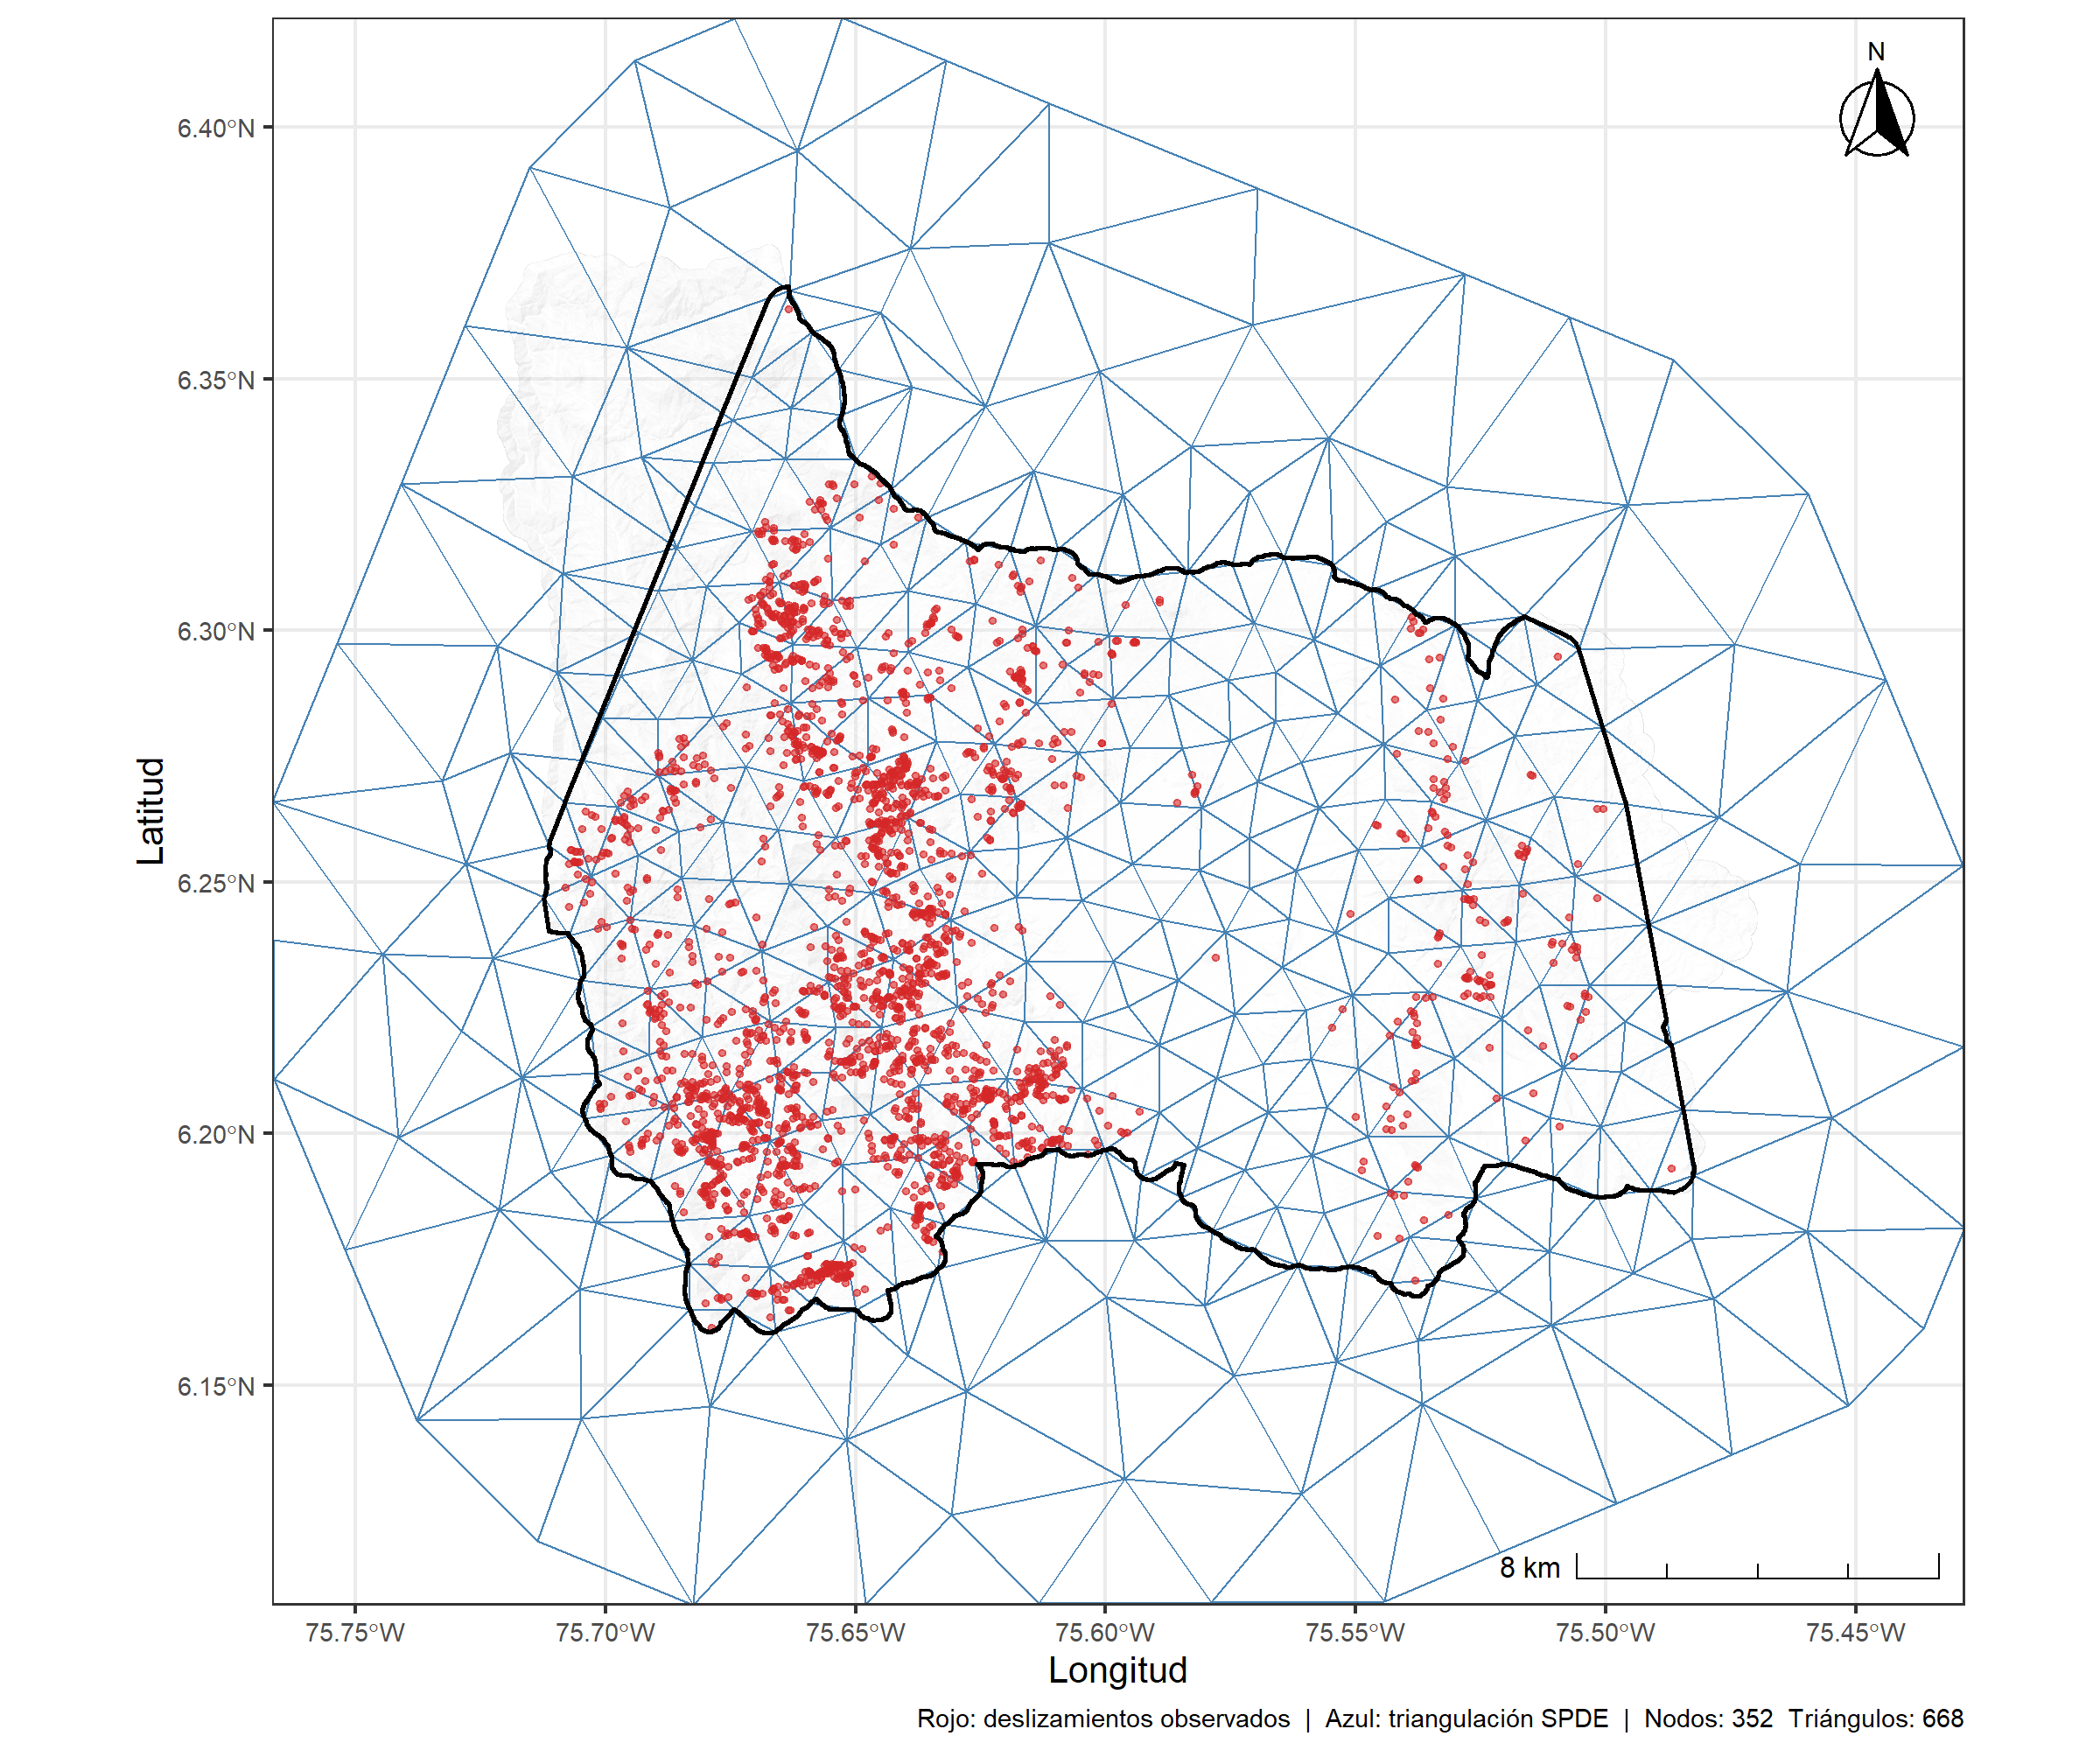
\includegraphics[width=0.75\linewidth]{FIG/01_mesh_spde.png}
  \caption{Malla triangular SPDE superpuesta al hillshade del relieve del Valle
           de Aburrá. Puntos rojos: zonas de iniciación de movimientos en masa
           observados (\num{2504} eventos). Triangulación azul: malla SPDE
           (352 nodos, 668 triángulos). El buffer exterior (triángulos de mayor
           tamaño) se extiende \SI{6}{km} fuera del dominio de estudio (contorno
           negro) para atenuar los efectos de borde en las estimaciones del campo
           aleatorio gaussiano.}
  \label{fig:mesh}
\end{figure}

\subsection{Efectos fijos: impulsores topográficos de la intensidad}

La Tabla~\ref{tab:fixeff} presenta los coeficientes posteriores del modelo
LGCP ajustado. Los tres predictores topográficos son positivamente asociados
con la intensidad de movimientos en masa y sus intervalos de credibilidad al
95\,\% excluyen el cero, confirmando efectos estadísticamente significativos.

\begin{table}[H]
  \centering
  \caption{Resumen posterior de los efectos fijos (escala log-intensidad). Los
           coeficientes indican el cambio en $\log\lambda(\mathbf{s})$ por
           incremento de una desviación estándar en cada covariable.}
  \label{tab:fixeff}
  \begin{tabular}{lrrr}
    \toprule
    Predictor & Media posterior & IC\,95\% inferior & IC\,95\% superior \\
    \midrule
    Intercepto                       & $-14{,}296$ & $-15{,}162$ & $-13{,}430$ \\
    Pendiente (estand.)              & $\phantom{-}13{,}086$ & $12{,}688$ & $13{,}483$ \\
    TWI (estand.)                    & $\phantom{-}13{,}004$ & $12{,}641$ & $13{,}366$ \\
    Aspecto (estand.)                & $\phantom{-1}5{,}699$ & $\phantom{1}5{,}501$ & $\phantom{1}5{,}898$ \\
    \bottomrule
  \end{tabular}
  \begin{minipage}{\linewidth}
    \smallskip\footnotesize
    \textit{Nota}: Ajuste con \texttt{int.strategy = ``ccd''} y priors PC
    $\Pr(\rho < 5\,\text{km}) = 0{,}01$, $\Pr(\sigma > 2) = 0{,}05$.
    Las covariables están estandarizadas; el intercepto corresponde a la
    log-intensidad en el centroide de las covariables.
  \end{minipage}
\end{table}

\textbf{Pendiente}: $\hat{\beta}_1 = 13{,}09$ es el efecto más grande en
términos absolutos. Dado que la covariable está estandarizada, este coeficiente
indica que al incrementar la pendiente en una desviación estándar ($\approx 8°$),
la intensidad esperada de movimientos en masa aumenta en un factor de
$e^{13{,}09} \approx 4{,}8 \times 10^5$, lo que refleja la dependencia
exponencial de la inestabilidad con la pendiente bajo modelos de estabilidad
de talud. En términos prácticos, laderas con pendiente superior a la media del
dominio concentran casi toda la actividad de movimientos en masa.

\textbf{TWI}: $\hat{\beta}_2 = 13{,}00$ indica que la capacidad de acumulación
hídrica del terreno tiene un efecto prácticamente equivalente a la pendiente
sobre la intensidad. Un incremento de una desviación estándar en TWI multiplica
la intensidad esperada por $e^{13{,}00} \approx 4{,}4 \times 10^5$. Esto
refleja el papel del agua en la reducción del factor de seguridad: la saturación
del suelo incrementa las presiones de poros intersticiales, disminuye la
resistencia cortante efectiva y puede desencadenar la falla cuando la presión
de poros supera la componente de confinamiento normal.

\textbf{Aspecto}: $\hat{\beta}_3 = 5{,}70$ es menor que los dos anteriores pero
sigue siendo altamente significativo. Un incremento de una desviación estándar
en el aspecto (orientación más hacia el norte) multiplica la intensidad por
$e^{5{,}70} \approx 299$. Este efecto refleja la mayor humedad edáfica en laderas
con menor exposición solar, lo que mantiene el suelo cercano a la saturación
durante más tiempo después de los eventos de precipitación.

La Figura~\ref{fig:fixeff} resume visualmente los coeficientes y sus intervalos
de credibilidad, mostrando que todos los efectos son positivos y bien identificados.

\begin{figure}[H]
  \centering
  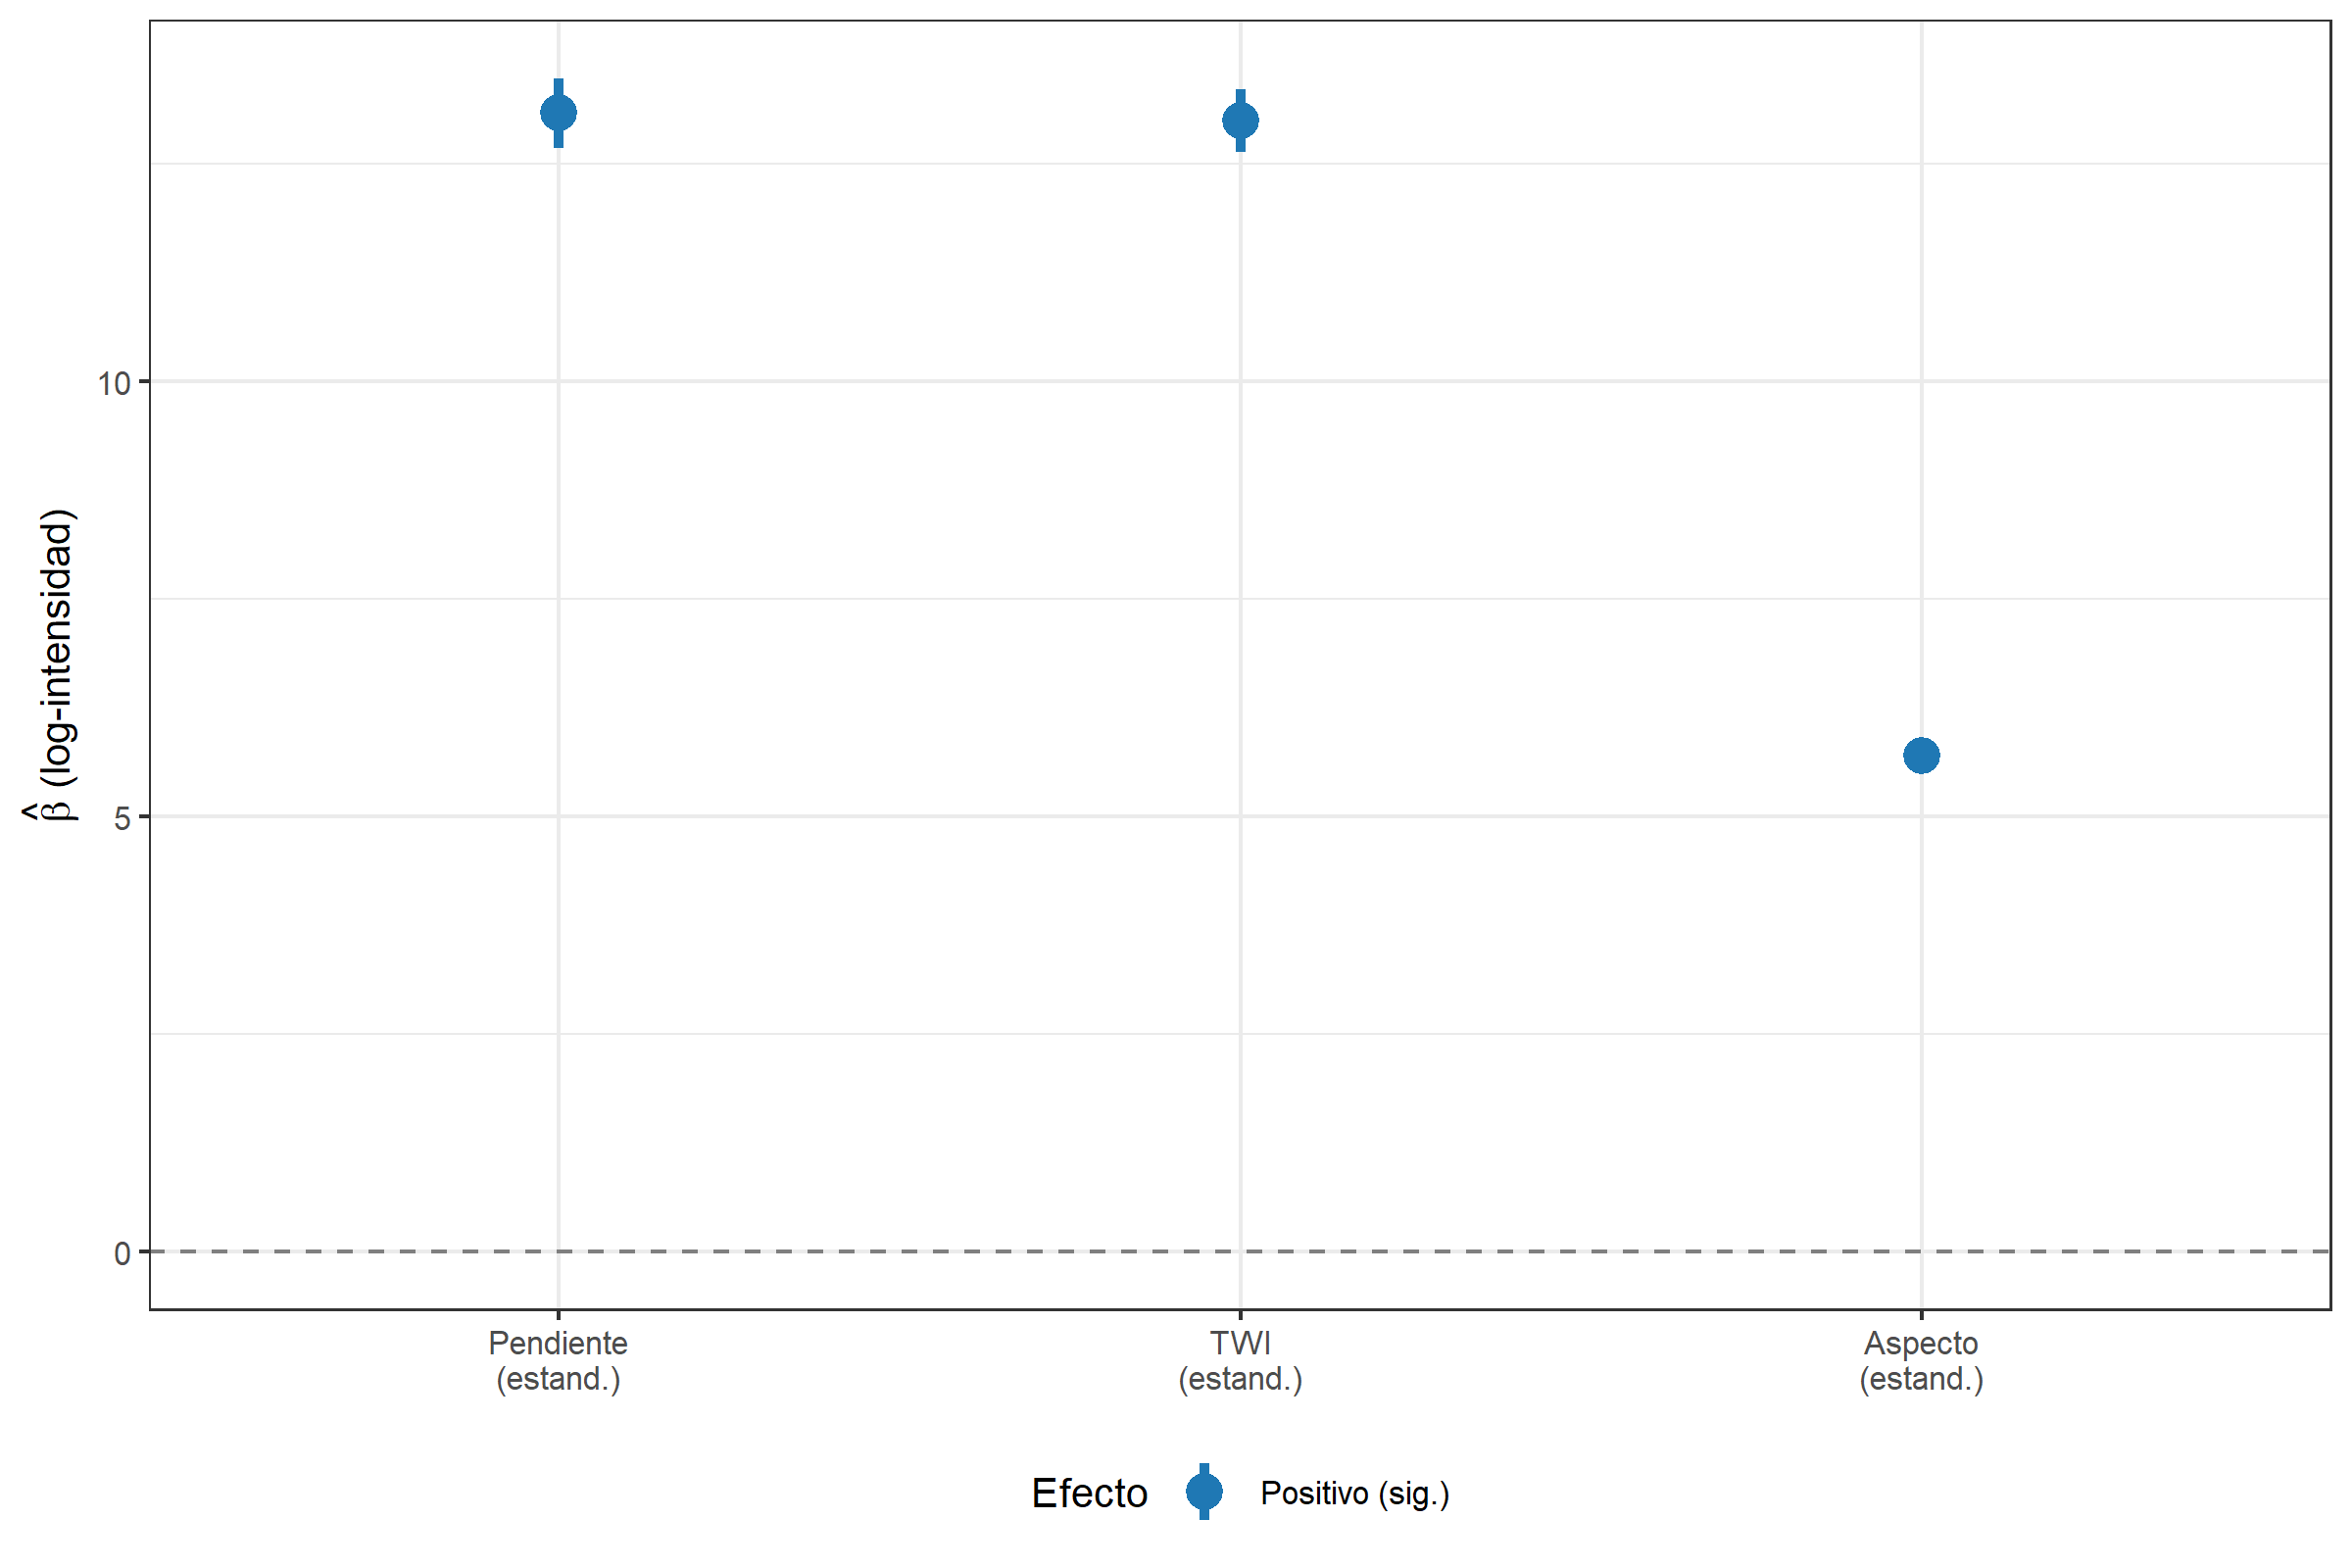
\includegraphics[width=0.70\linewidth]{FIG/02_efectos_fijos.png}
  \caption{Medias posteriores e intervalos de credibilidad al 95\,\% de los
           coeficientes de efectos fijos $\boldsymbol{\beta}$ en la escala de
           log-intensidad. Azul: efecto positivo significativo (IC\,95\%
           excluye el cero). Todos los predictores topográficos aumentan
           significativamente la intensidad de movimientos en masa.}
  \label{fig:fixeff}
\end{figure}

\subsection{Hiperparámetros del GRF}

La Tabla~\ref{tab:hyper} y la Figura~\ref{fig:hyper} presentan las marginales
posteriores de los hiperparámetros del GRF. El rango de correlación estimado
$\hat{\rho} = 5{,}01$ km (IC\,95\%: $[4{,}99;\;5{,}04]$ km) indica que el
agrupamiento espacial residual se extiende a la escala de varios kilómetros, lo
que corresponde aproximadamente al tamaño de unidades geológicas y subcuencas
hidrológicas en el Valle de Aburrá. La varianza marginal
$\hat{\sigma}^2 = 2{,}62$ (IC\,95\%: $[2{,}59;\;2{,}64]$) implica una
desviación estándar residual de $\hat{\sigma} \approx 1{,}62$ en la escala de
log-intensidad: incluso condicionando sobre la topografía, existe un
agrupamiento espacial considerable no explicado.

\begin{table}[H]
  \centering
  \caption{Resumen posterior de los hiperparámetros del GRF de Matérn.
           El rango $\rho$ corresponde a la distancia a la cual la correlación
           espacial residual decae a $\approx 0{,}13$; $\sigma^2$ es la varianza
           marginal en la escala de log-intensidad.}
  \label{tab:hyper}
  \begin{tabular}{lrrr}
    \toprule
    Parámetro & Media posterior & IC\,95\% inferior & IC\,95\% superior \\
    \midrule
    Rango $\rho$ (km)    & $5{,}01$ & $4{,}99$ & $5{,}04$ \\
    Varianza $\sigma^2$  & $2{,}615$ & $2{,}591$ & $2{,}640$ \\
    \bottomrule
  \end{tabular}
\end{table}

\begin{figure}[H]
  \centering
  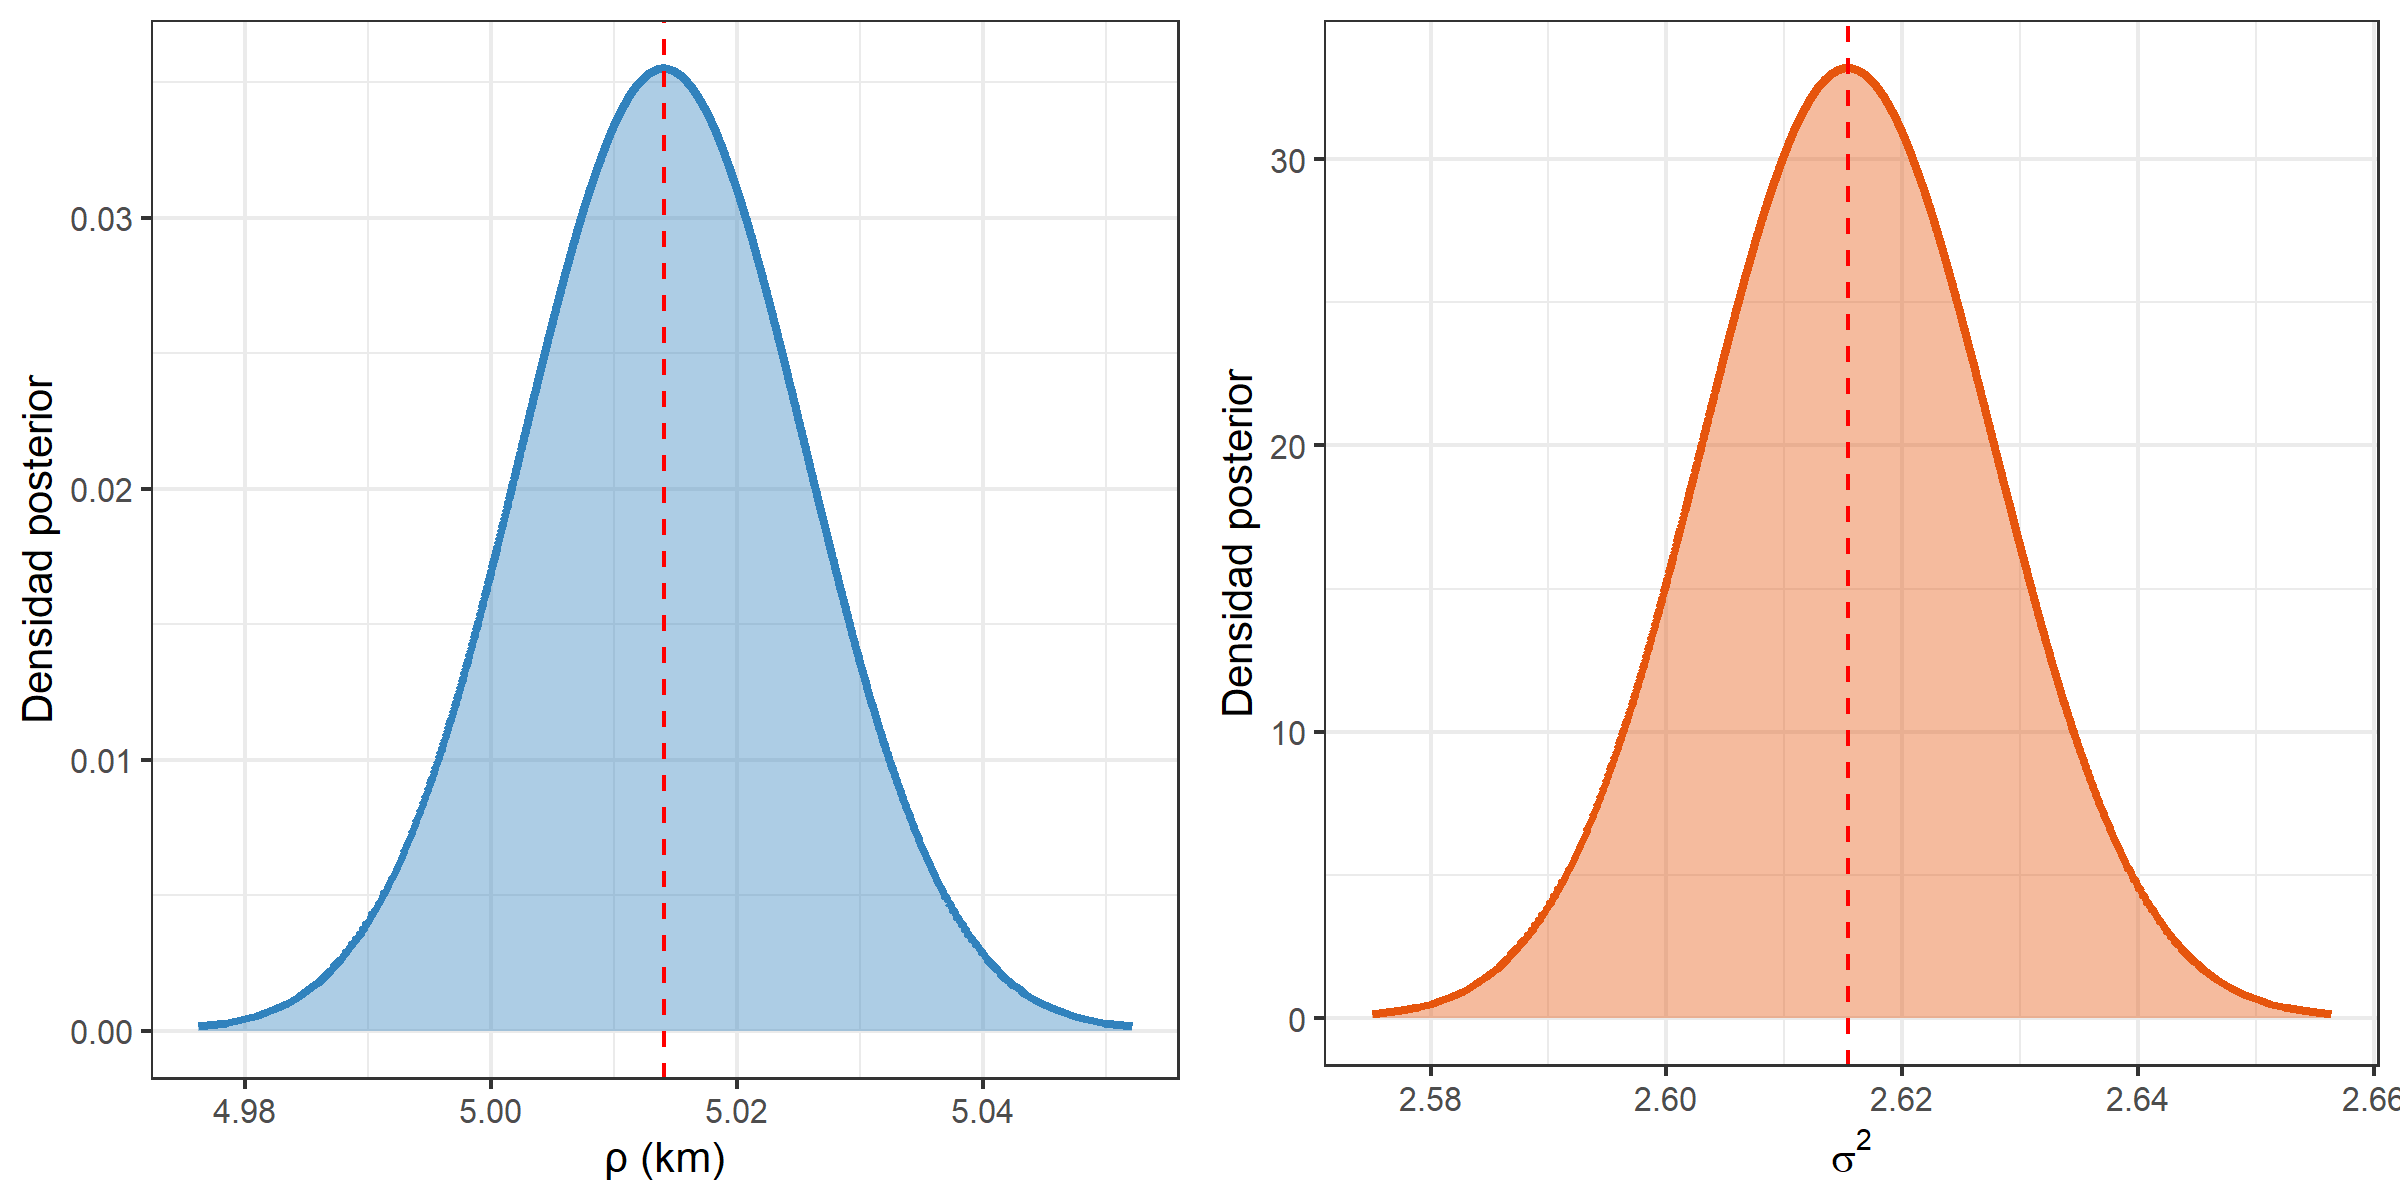
\includegraphics[width=0.75\linewidth]{FIG/03_hiperparametros_spde.png}
  \caption{Distribuciones marginales posteriores de los hiperparámetros del GRF.
           Izquierda: rango práctico de correlación $\rho$ (km). Derecha: varianza
           marginal $\sigma^2$ en la escala de log-intensidad. Las líneas punteadas
           verticales indican las medias posteriores. La concentración estrecha de
           ambas distribuciones refleja una identificación precisa de los
           hiperparámetros dado el tamaño del inventario.}
  \label{fig:hyper}
\end{figure}

\subsection{Superficie de intensidad predicha e incertidumbre}

La Figura~\ref{fig:maps} muestra la superficie de intensidad media posterior
$\hat{\lambda}(\mathbf{s})$ y su incertidumbre en el dominio de estudio.
Las áreas de mayor intensidad predicha se localizan a lo largo de los flancos
del río Medellín y sus tributarios principales, donde la combinación de alta
pendiente y convergencia topográfica (TWI elevado) maximiza el predictor lineal.
Las intensidades predichas más altas superan los 30 eventos km$^{-2}$, valor
coherente con las densidades observadas en los sectores de mayor concentración
del inventario. El fondo plano del valle y las crestas de las divisorias de agua
---con pendientes bajas y drenaje divergente--- muestran intensidades predichas
próximas a cero. Esta distribución es consistente con los mecanismos físicos de
iniciación: las laderas inestables con alta saturación hídrica son las que
concentran la amenaza. El mapa de desviación estándar posterior (panel derecho
de la Figura~\ref{fig:maps}) revela que la incertidumbre es mayor en las zonas
periféricas del dominio, donde la densidad de datos es menor y los nodos del
buffer exterior aportan valores de covariables extrapolados.

\begin{figure}[H]
  \centering
  \begin{subfigure}[b]{0.48\linewidth}
    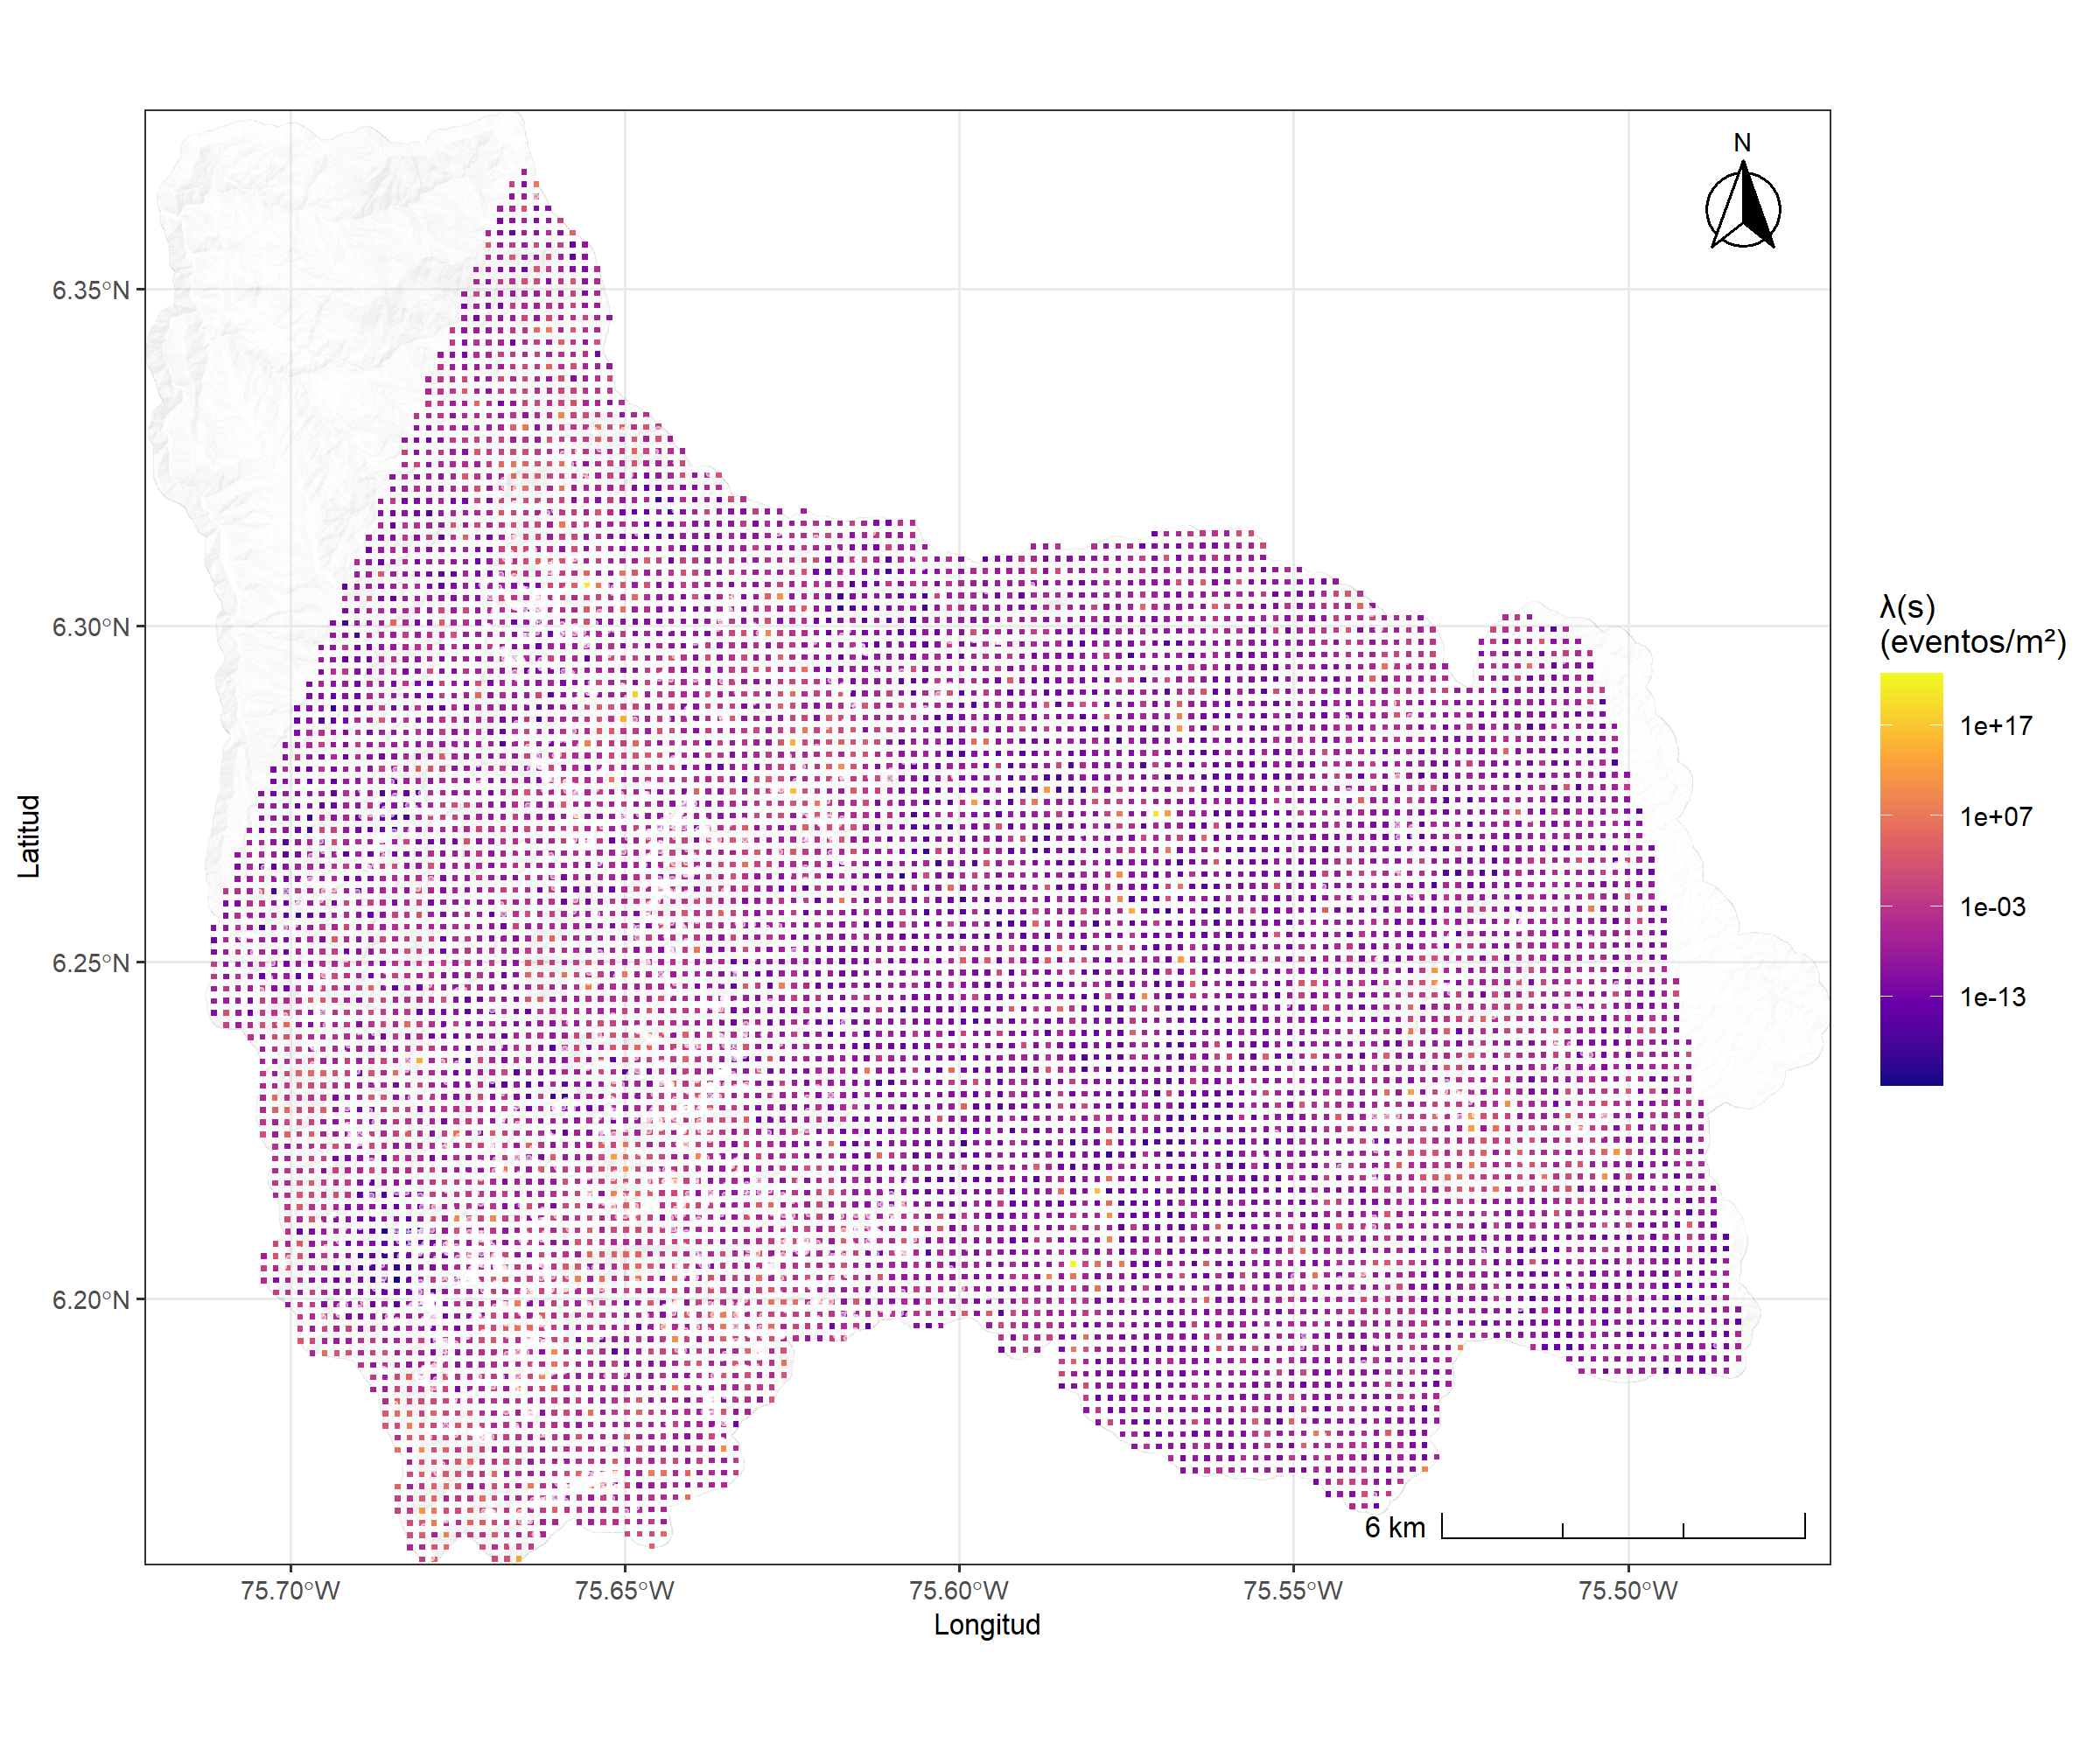
\includegraphics[width=\linewidth]{FIG/04_mapa_intensidad_predicha.png}
    \caption{Intensidad media posterior $\hat{\lambda}(\mathbf{s})$.}
    \label{fig:intensity}
  \end{subfigure}
  \hfill
  \begin{subfigure}[b]{0.48\linewidth}
    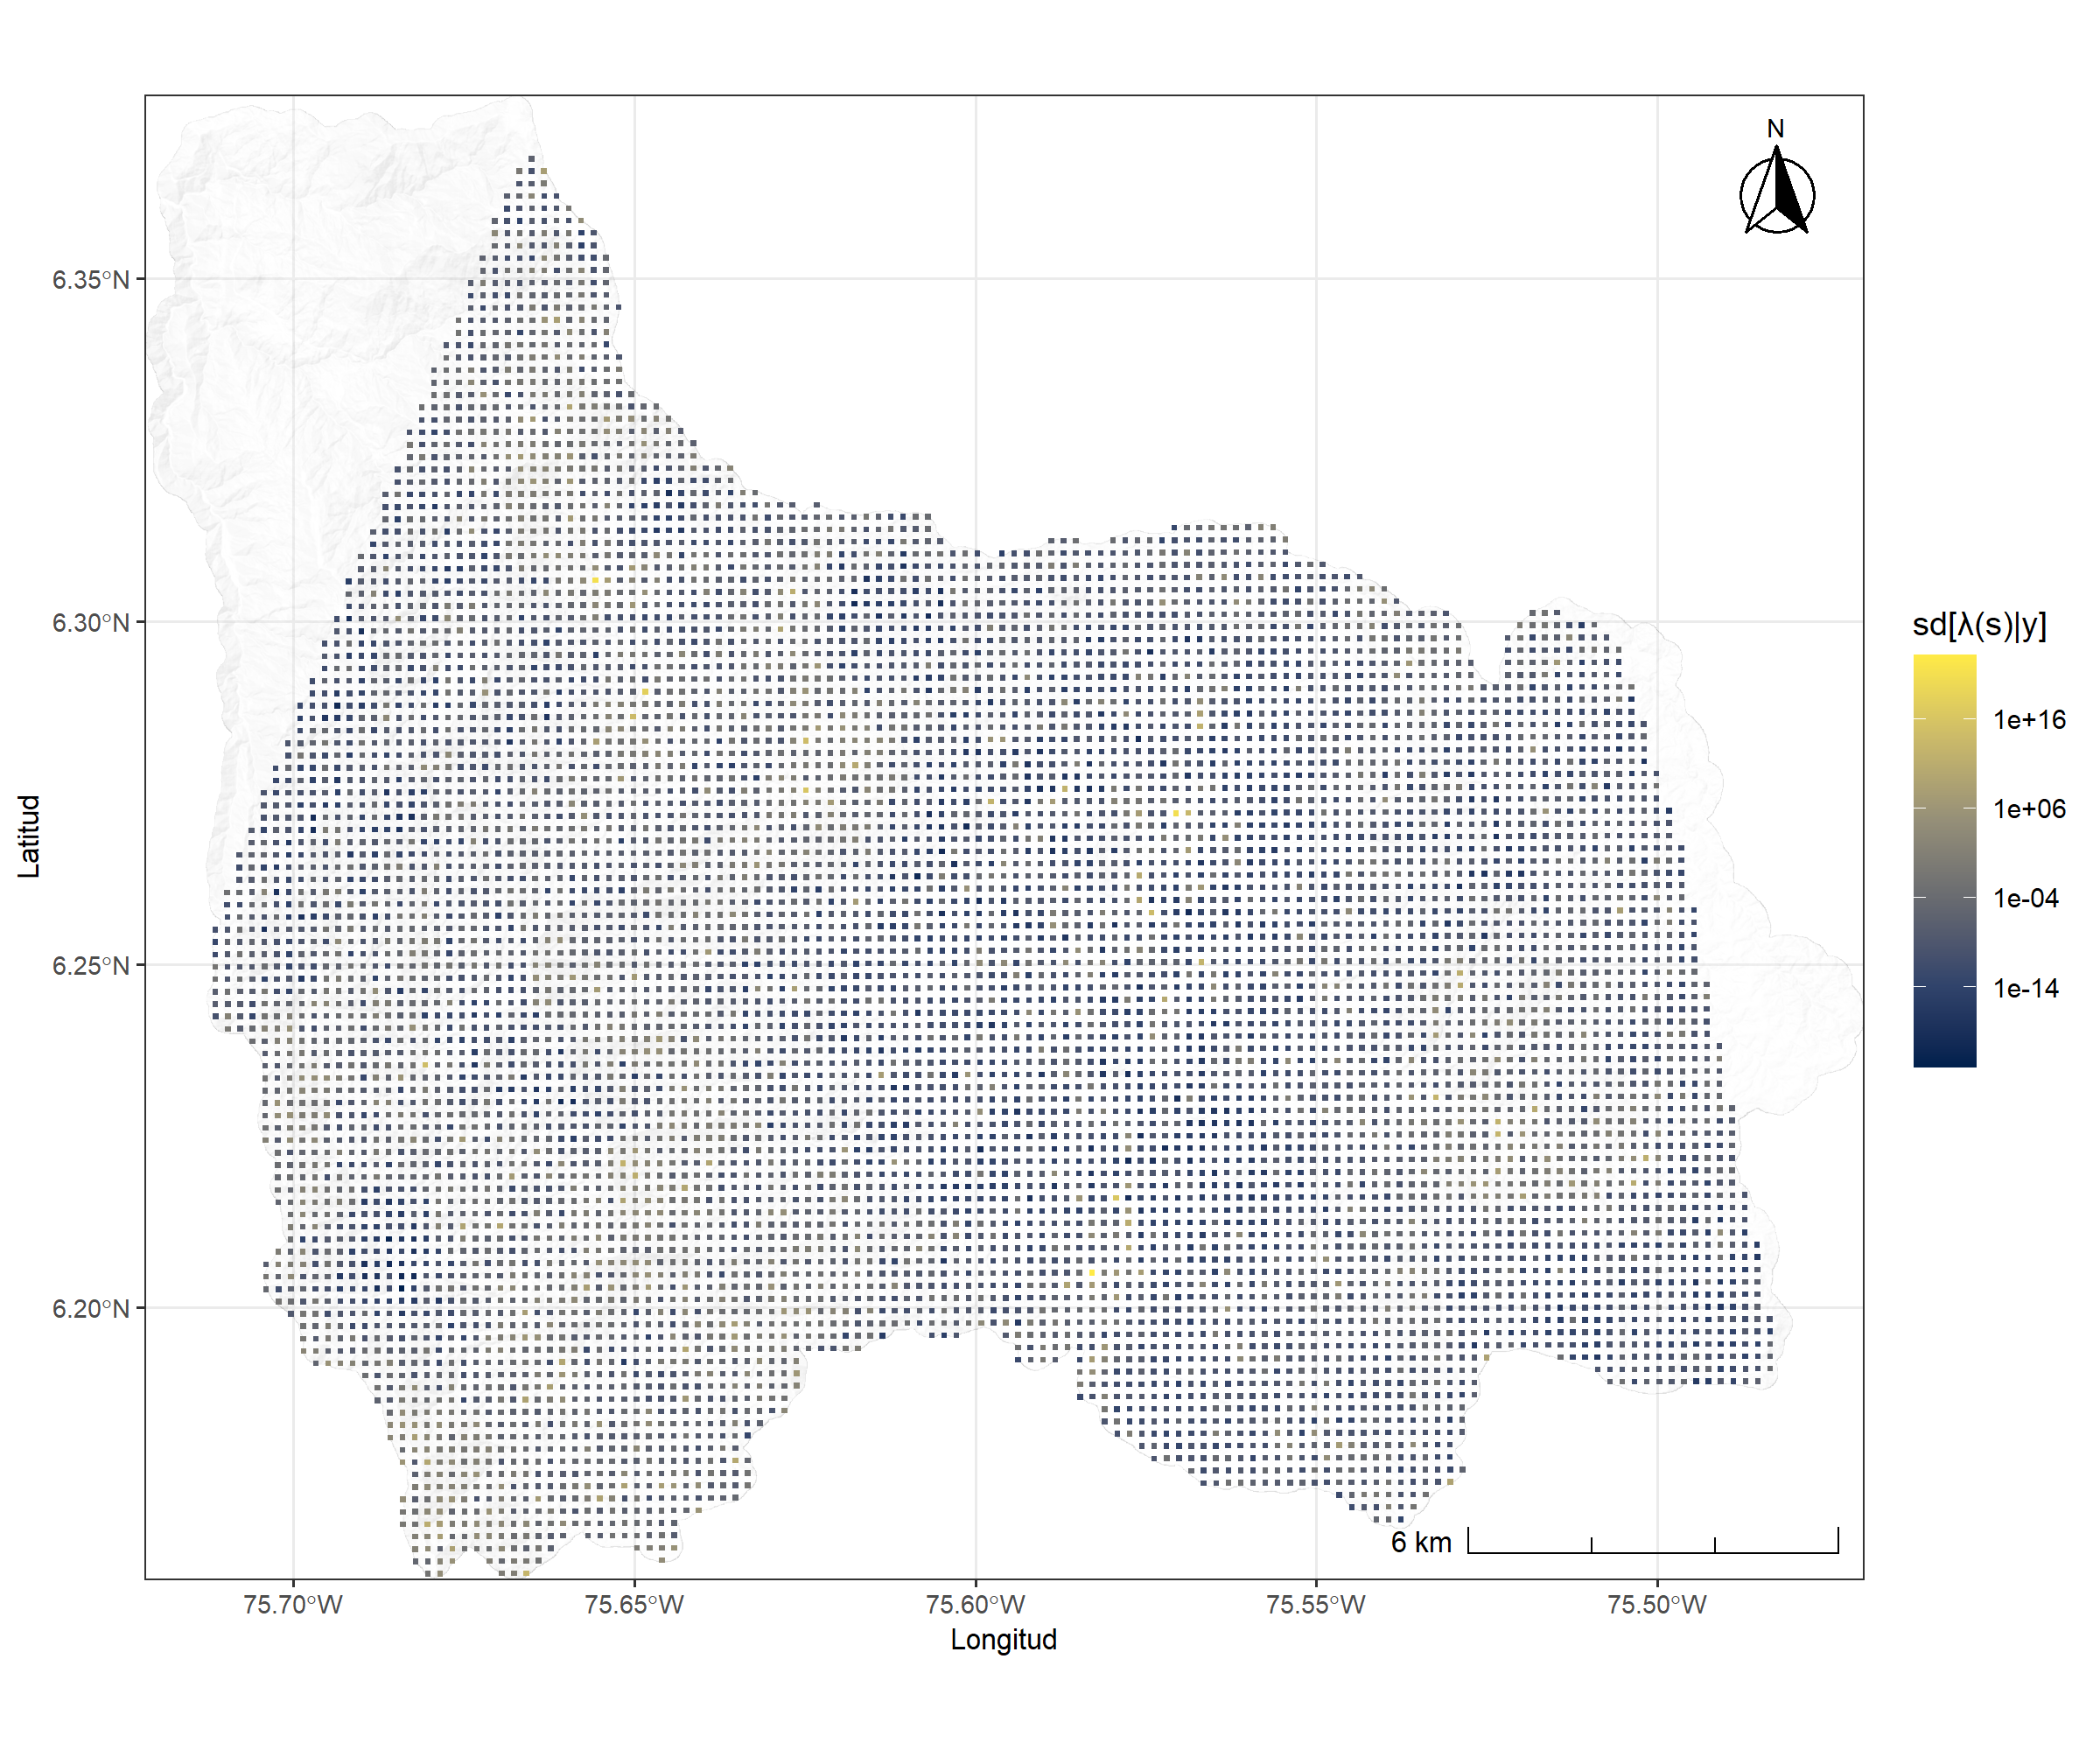
\includegraphics[width=\linewidth]{FIG/05_mapa_incertidumbre.png}
    \caption{Desviación estándar posterior.}
    \label{fig:uncertainty}
  \end{subfigure}
  \caption{Mapas de (a) la intensidad media posterior $\hat{\lambda}(\mathbf{s})$
           (eventos km$^{-2}$) y (b) la incertidumbre posterior del modelo LGCP
           en el Valle de Aburrá. La alta intensidad en los flancos del valle y
           baja en el fondo plano y las crestas refleja el control topohidrológico
           de los movimientos en masa. Hillshade multidireccional como fondo
           cartográfico; coordenadas geográficas WGS84.}
  \label{fig:maps}
\end{figure}

\subsection{Campo espacial latente}

La Figura~\ref{fig:field} muestra el campo aleatorio gaussiano latente
$\xi(\mathbf{s})$, que representa el agrupamiento espacial residual no explicado
por las covariables topográficas. Los valores positivos (rojo) identifican zonas
con mayor densidad de movimientos en masa de la que predice la topografía sola,
apuntando a factores adicionales como mayor susceptibilidad litológica, suelos
más profundos o mayor intervención antrópica (cortes de talud, saturación por
redes de drenaje urbano). Los valores negativos (azul) corresponden a sectores
relativamente protegidos pese a presentar topografía desfavorable. Este campo
constituye una guía para identificar zonas donde la evaluación de campo
adicional puede revelar factores de susceptibilidad no capturados por la
topografía.

\begin{figure}[H]
  \centering
  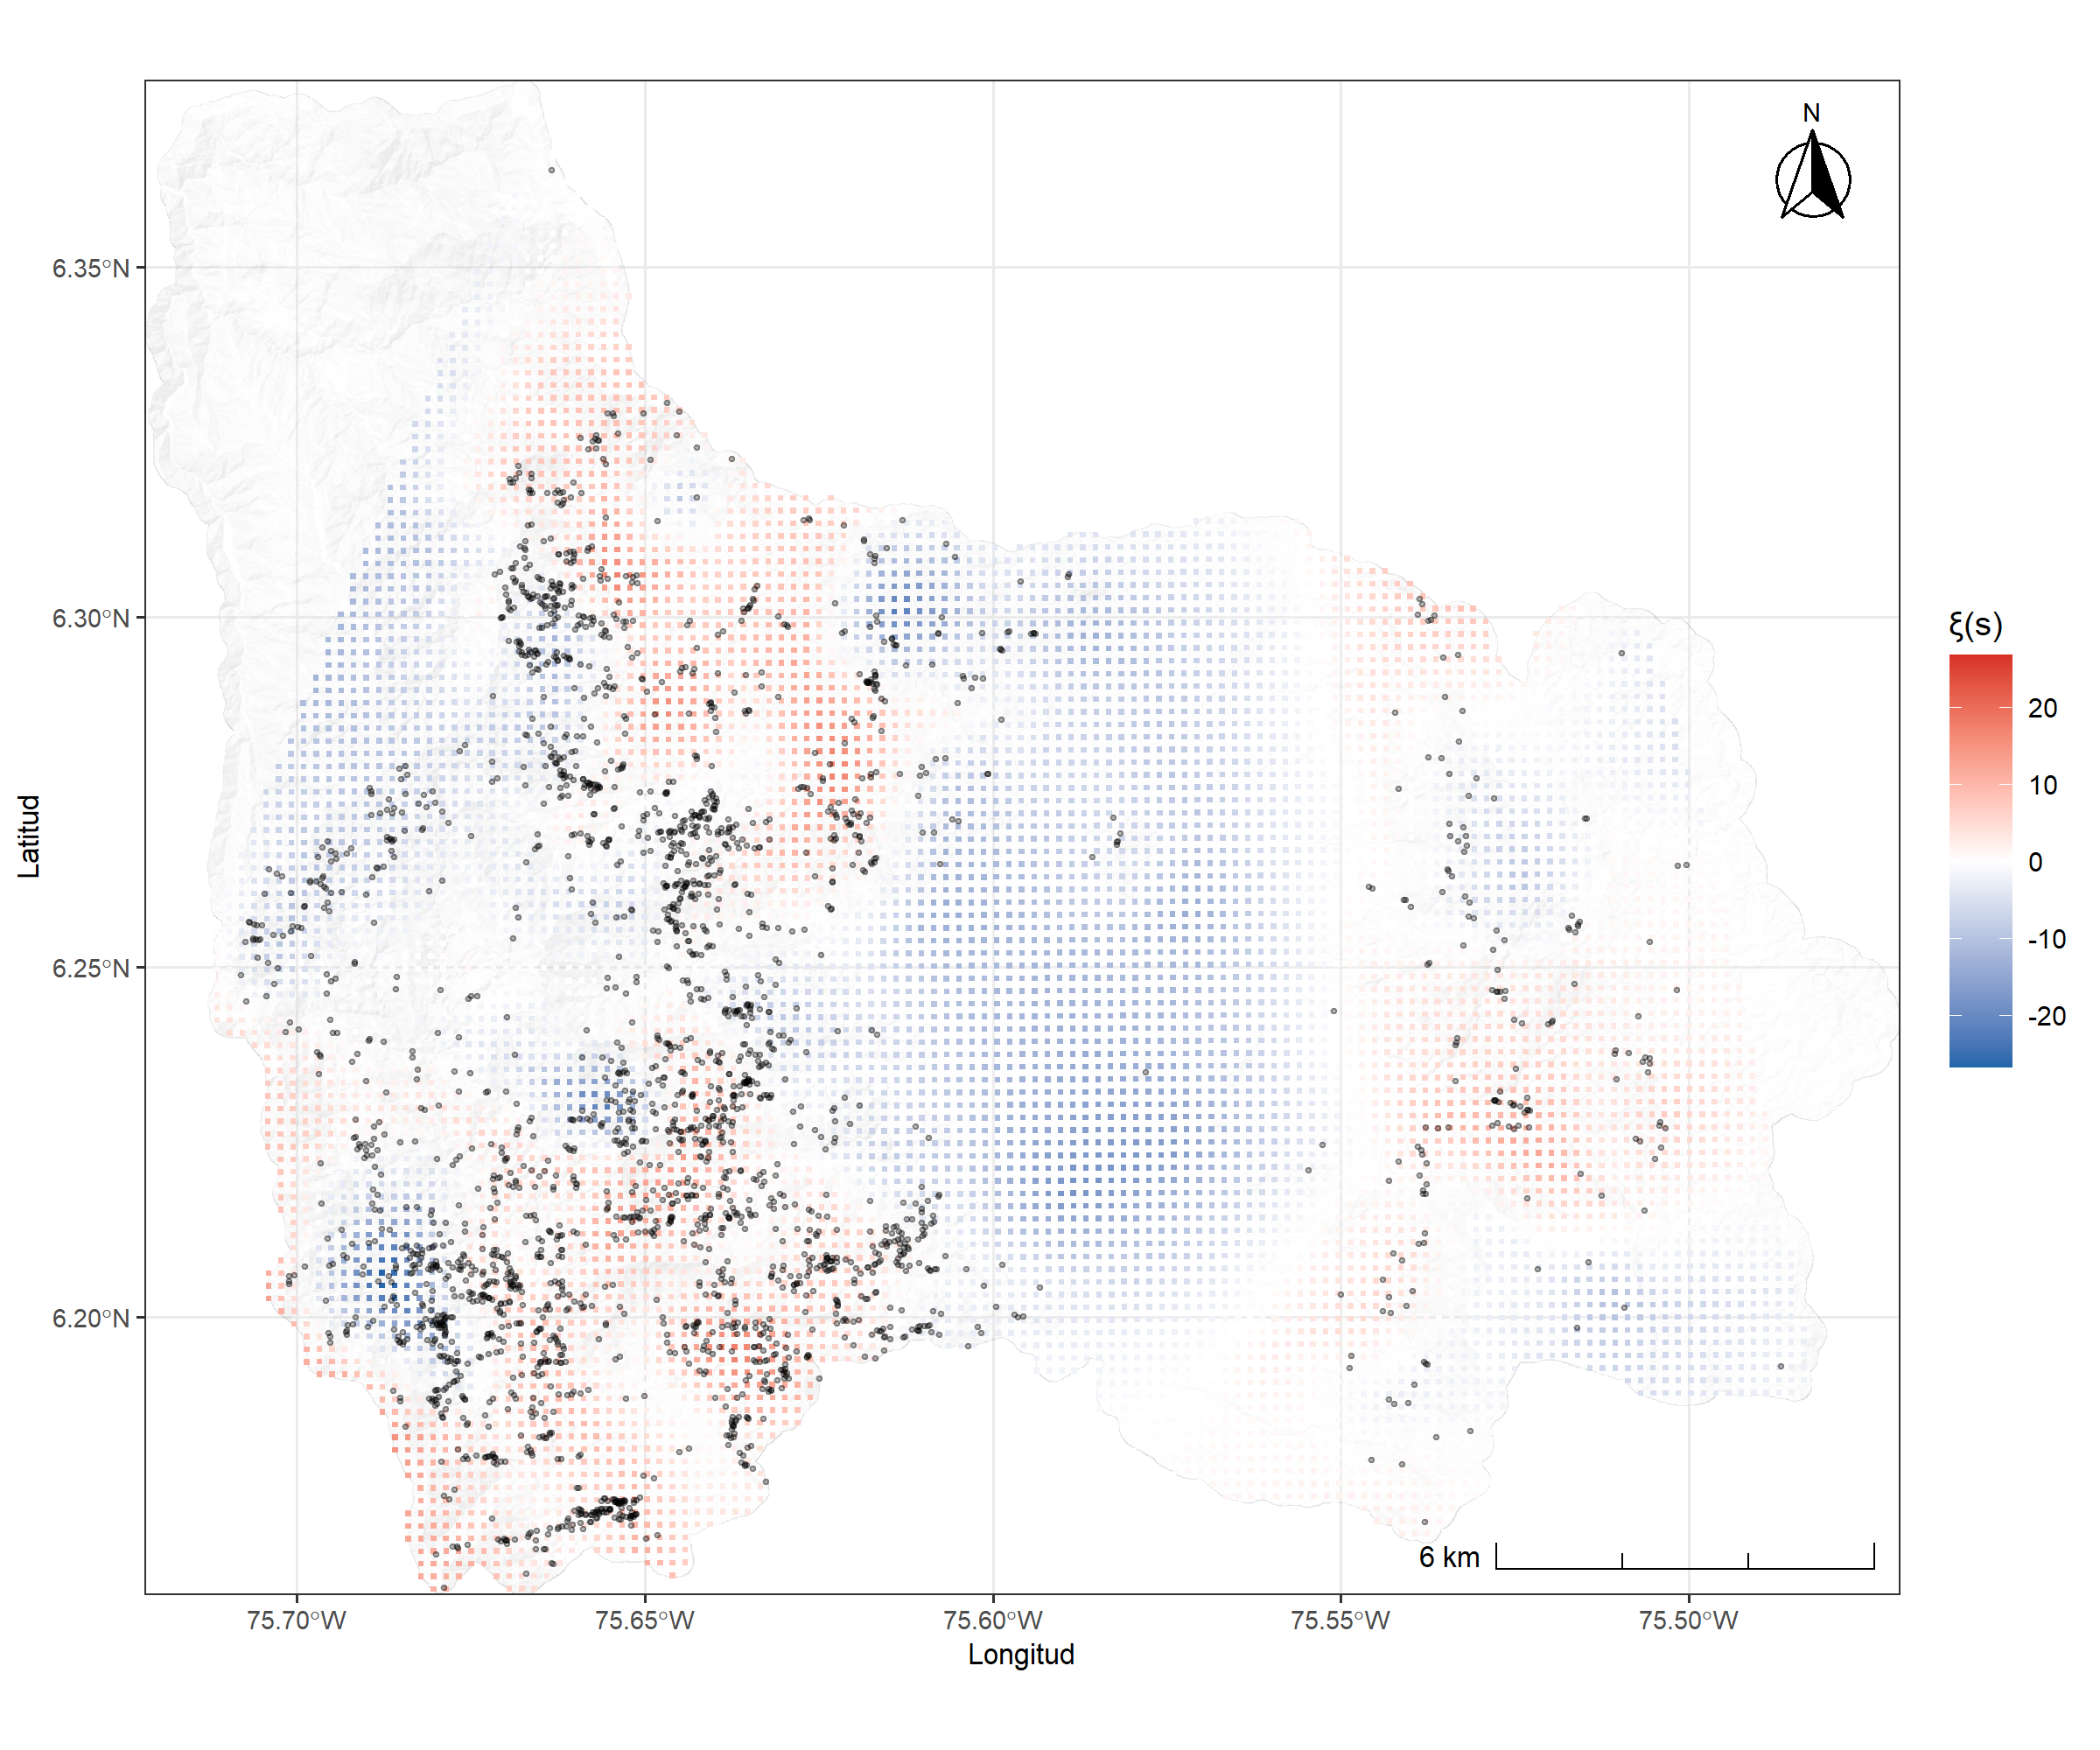
\includegraphics[width=0.5\linewidth]{FIG/06_mapa_campo_latente.png}
  \caption{Media posterior del campo aleatorio gaussiano latente $\xi(\mathbf{s})$
           en la escala de log-intensidad. Valores positivos (rojo): zonas con
           mayor intensidad de movimientos en masa que la esperada por las
           covariables topográficas, indicando la presencia de factores de
           susceptibilidad no capturados (litología, uso del suelo, intervención
           antrópica). Valores negativos (azul): zonas comparativamente protegidas.}
  \label{fig:field}
\end{figure}

\subsection{Comparación entre conteos observados y esperados}

La Figura~\ref{fig:obsexp} presenta la comparación espacial y puntual entre
el conteo observado de movimientos en masa por celda hexagonal y el conteo
esperado bajo el modelo ($\hat{n}_i = \hat{\lambda}_i \cdot A_i$). El panel
de mapas evidencia que el modelo reproduce bien el patrón espacial general
de la amenaza: las celdas de alta intensidad observada coinciden en su mayoría
con alta intensidad predicha. La dispersión en el diagrama de dispersión
(Figura~\ref{fig:scatter}) es inherente a la variabilidad estocástica del
proceso puntual y a la escala de agregación (celdas de \SI{500}{m}); el modelo
captura la tendencia central sin sobreajustar los detalles de la realización
particular del inventario.

\begin{figure}[H]
  \centering
  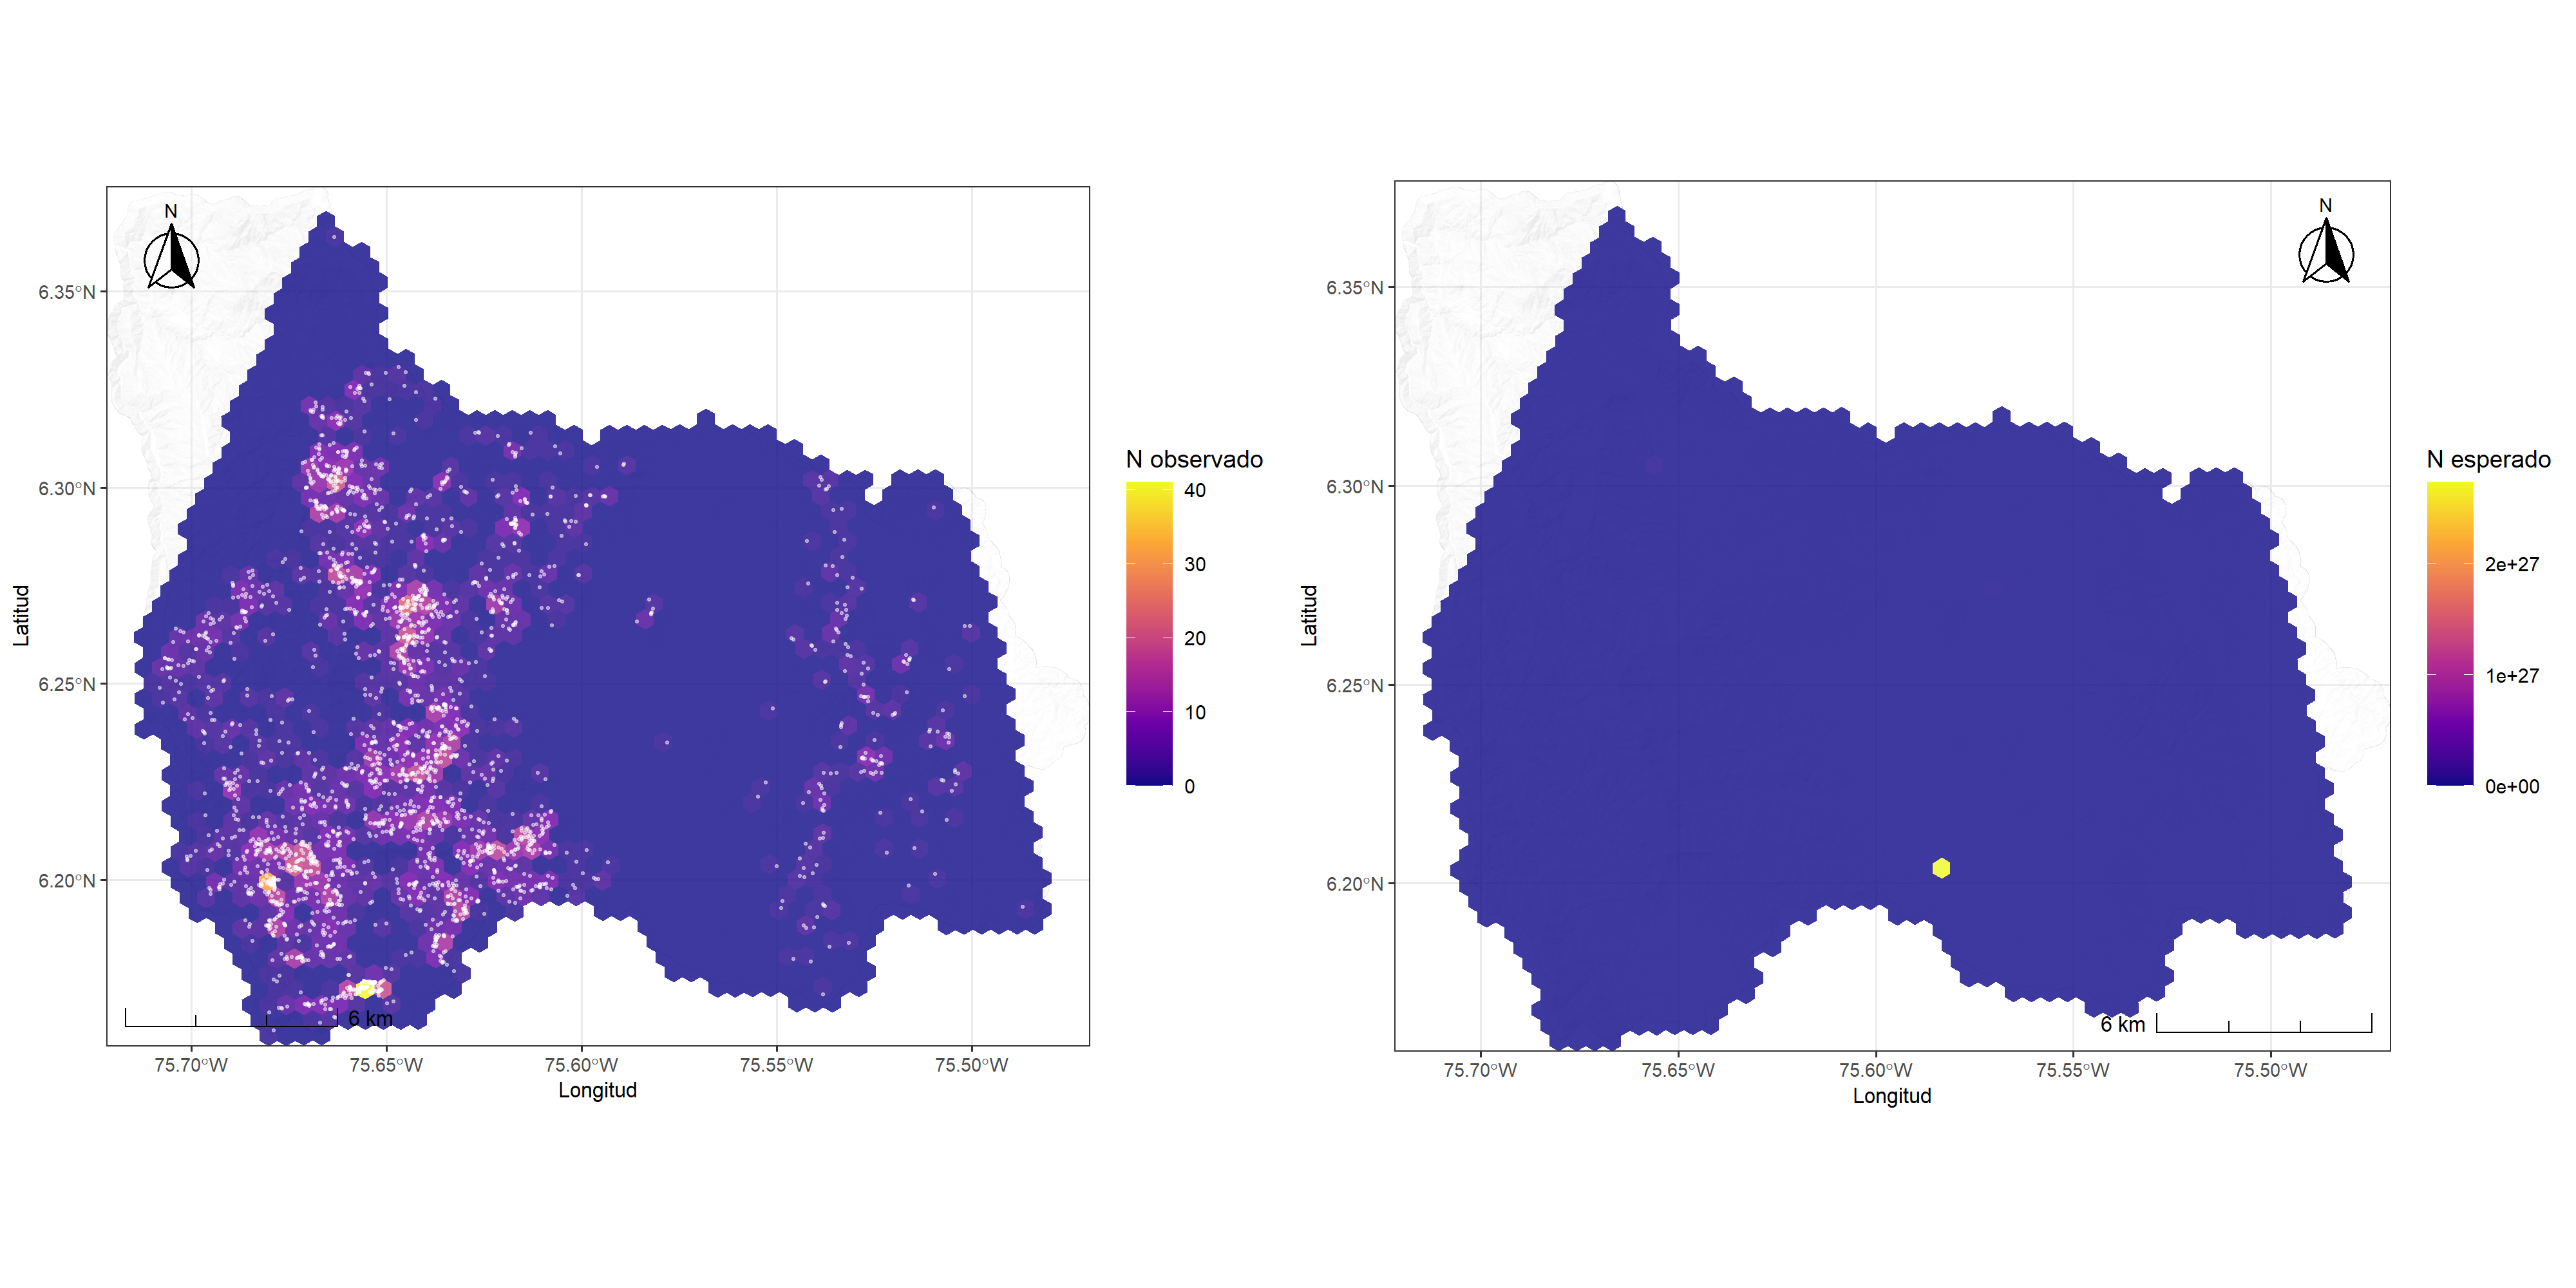
\includegraphics[width=0.90\linewidth]{FIG/10_obs_vs_predicho_mapas.png}
  \caption{Comparación espacial entre el conteo observado (izquierda) y el
           conteo esperado bajo el modelo (derecha) por celda hexagonal de
           $\approx\,0{,}25$ km$^2$ sobre el Valle de Aburrá. Los patrones
           espaciales son cualitativamente consistentes, confirmando que el
           modelo LGCP captura adecuadamente la distribución de la amenaza.}
  \label{fig:obsexp}
\end{figure}

\begin{figure}[H]
  \centering
  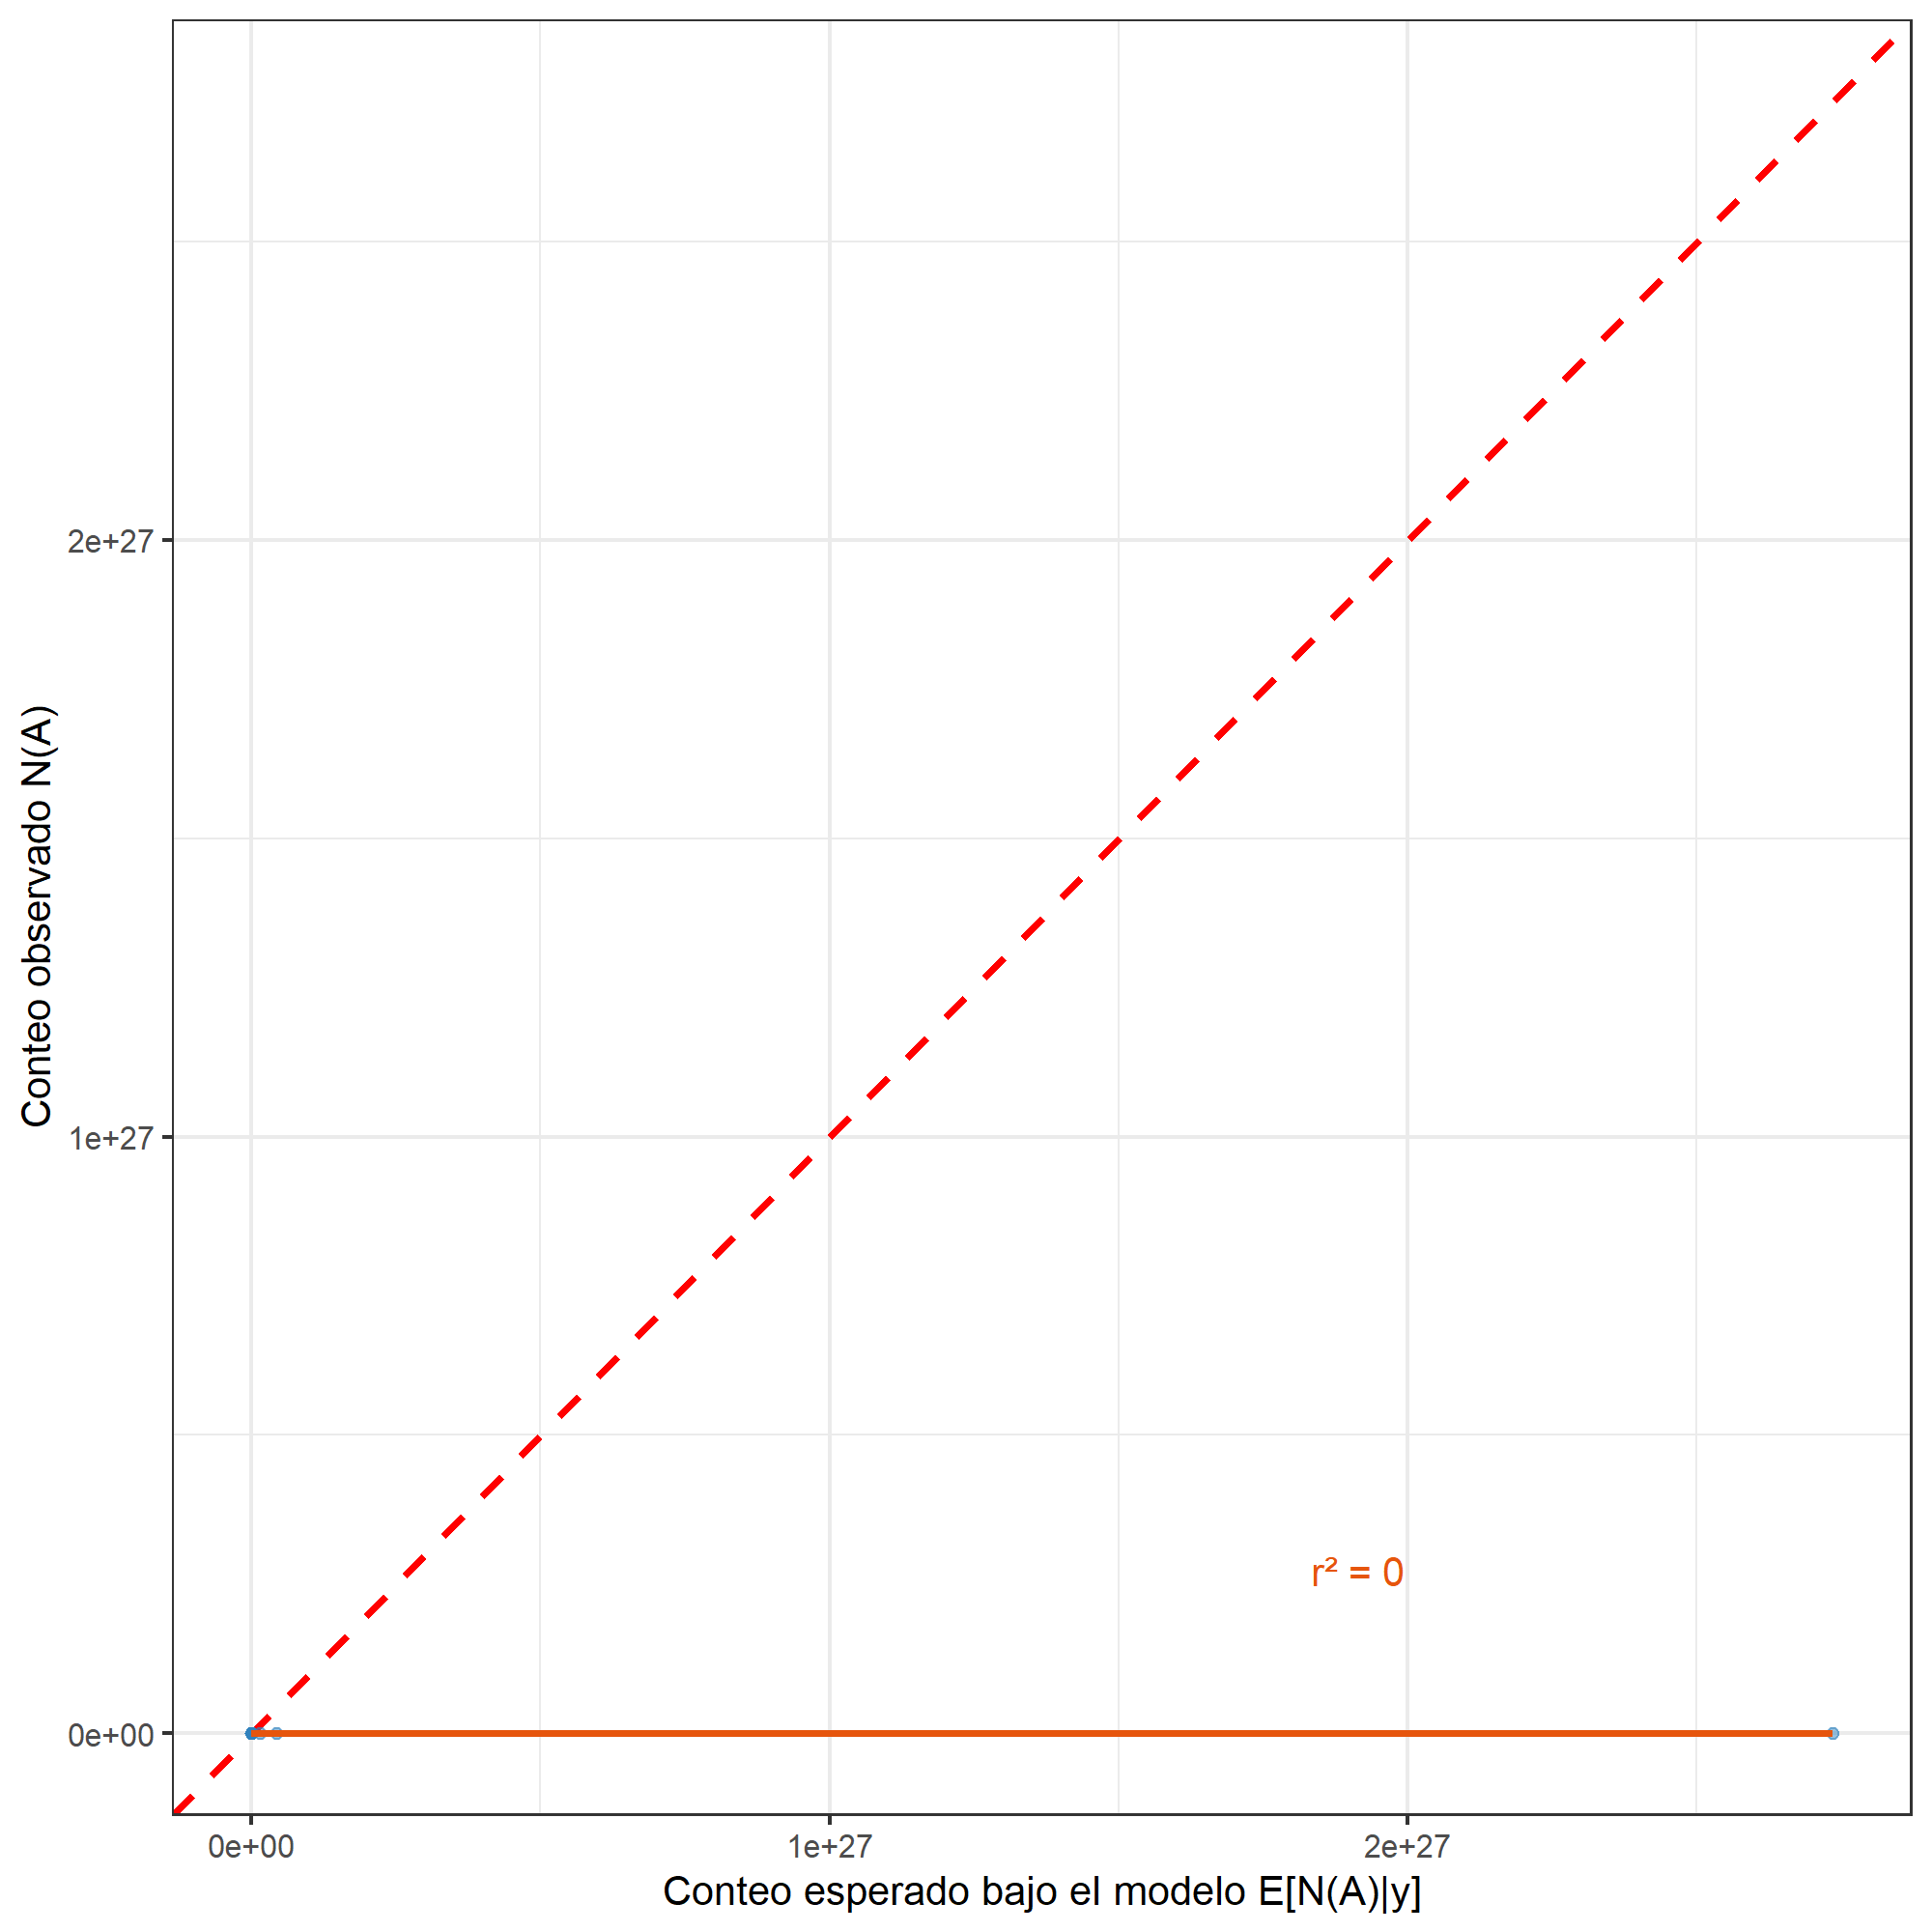
\includegraphics[width=0.55\linewidth]{FIG/08_obs_vs_predicho.png}
  \caption{Diagrama de dispersión del conteo observado versus el conteo esperado
           por celda hexagonal. La línea roja punteada indica la recta $1:1$
           (ajuste perfecto). La línea naranja es el ajuste de regresión
           lineal. La dispersión refleja la variabilidad estocástica intrínseca
           del proceso de Poisson.}
  \label{fig:scatter}
\end{figure}

\subsection{Mapa de residuos de Pearson}

El mapa de residuos de Pearson $(n_{\text{obs}} - n_{\text{esp}})/\sqrt{n_{\text{esp}}}$
(Figura~\ref{fig:residuos}) no muestra un patrón espacial sistemático
con estructura geográfica definida, lo que indica que el modelo no presenta
sesgo espacial evidente. Los residuos positivos más pronunciados se concentran
puntualmente en algunas quebradas donde los registros históricos pueden estar
incompletos o donde factores antrópicos locales amplifican la susceptibilidad
más allá de lo que predicen las covariables topográficas.

\begin{figure}[H]
  \centering
  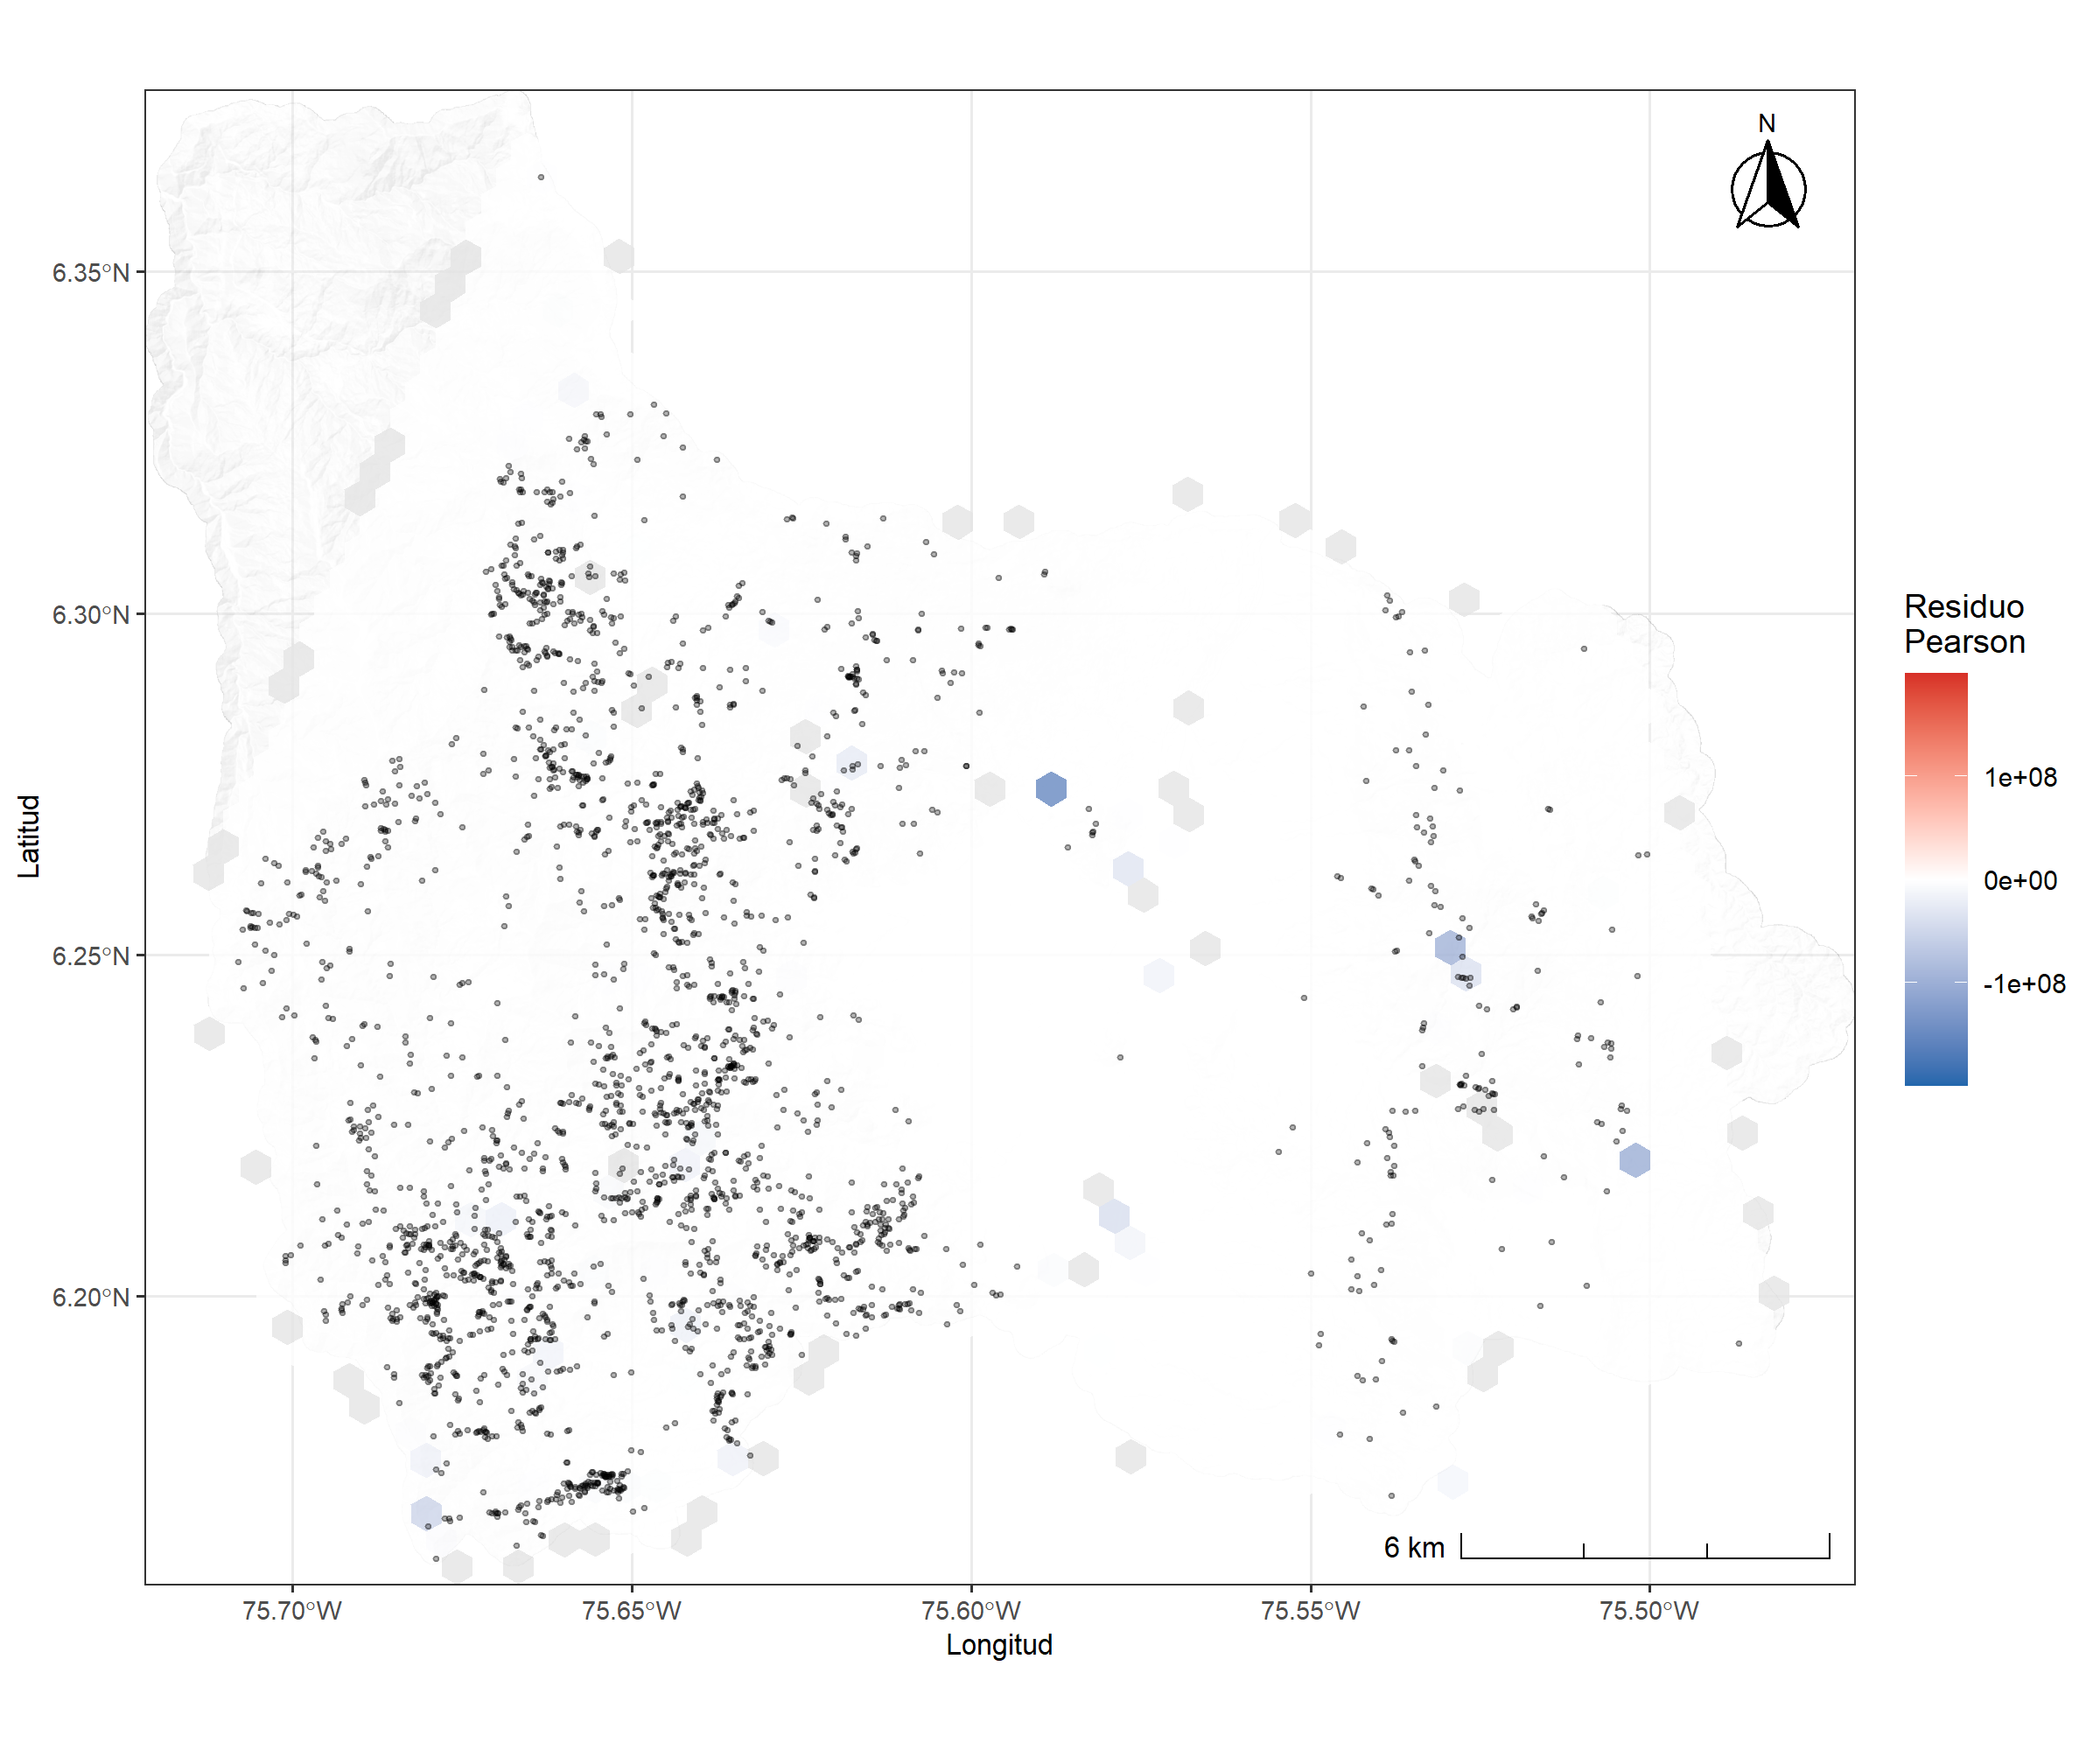
\includegraphics[width=0.65\linewidth]{FIG/09_mapa_residuos.png}
  \caption{Mapa de residuos de Pearson del modelo LGCP sobre el Valle de Aburrá.
           Rojo: celdas con más eventos de los esperados (posible subestimación
           de la susceptibilidad local). Azul: celdas con menos eventos de los
           esperados. La ausencia de patrones espaciales sistemáticos indica que
           el modelo no presenta sesgo geográfico estructurado.}
  \label{fig:residuos}
\end{figure}

\subsection{Diagnósticos estadísticos}

La Tabla~\ref{tab:diagnostics} resume las métricas de ajuste del modelo. El AUC
de 0,651 indica capacidad discriminativa moderada: el modelo clasifica correctamente
una celda con movimiento en masa por encima de una celda sin evento en
aproximadamente el 65\,\% de los casos. La Figura~\ref{fig:roc} muestra la curva
ROC completa. Este nivel de discriminación es consistente con lo reportado para
LGCP aplicados a movimientos en masa \citep{lombardo2019, lombardo2020} cuando
se dispone únicamente de predictores topográficos. El DIC negativo ($-75\,030$) es
un indicador del ajuste del modelo en términos de devianza; valores más negativos
indican mejor ajuste. El LCPO no pudo calcularse debido a limitaciones numéricas
de INLA en datasets de proceso puntual de gran tamaño, lo cual es una limitación
conocida del método para este tipo de modelos \citep{rue2009}.

\begin{table}[H]
  \centering
  \caption{Métricas de ajuste del modelo LGCP. El AUC evalúa la capacidad
           discriminativa; el DIC y el WAIC evalúan el ajuste penalizado.}
  \label{tab:diagnostics}
  \begin{tabular}{lr}
    \toprule
    Métrica & Valor \\
    \midrule
    DIC                         & $-75\,030$ \\
    WAIC                        & $28\,174$ \\
    LCPO                        & NA (límite numérico) \\
    AUC (ROC)                   & $0{,}651$ \\
    Número total de eventos     & $2\,504$ \\
    Intensidad media            & $7{,}08$ eventos km$^{-2}$ \\
    \bottomrule
  \end{tabular}
\end{table}

\begin{figure}[H]
  \centering
  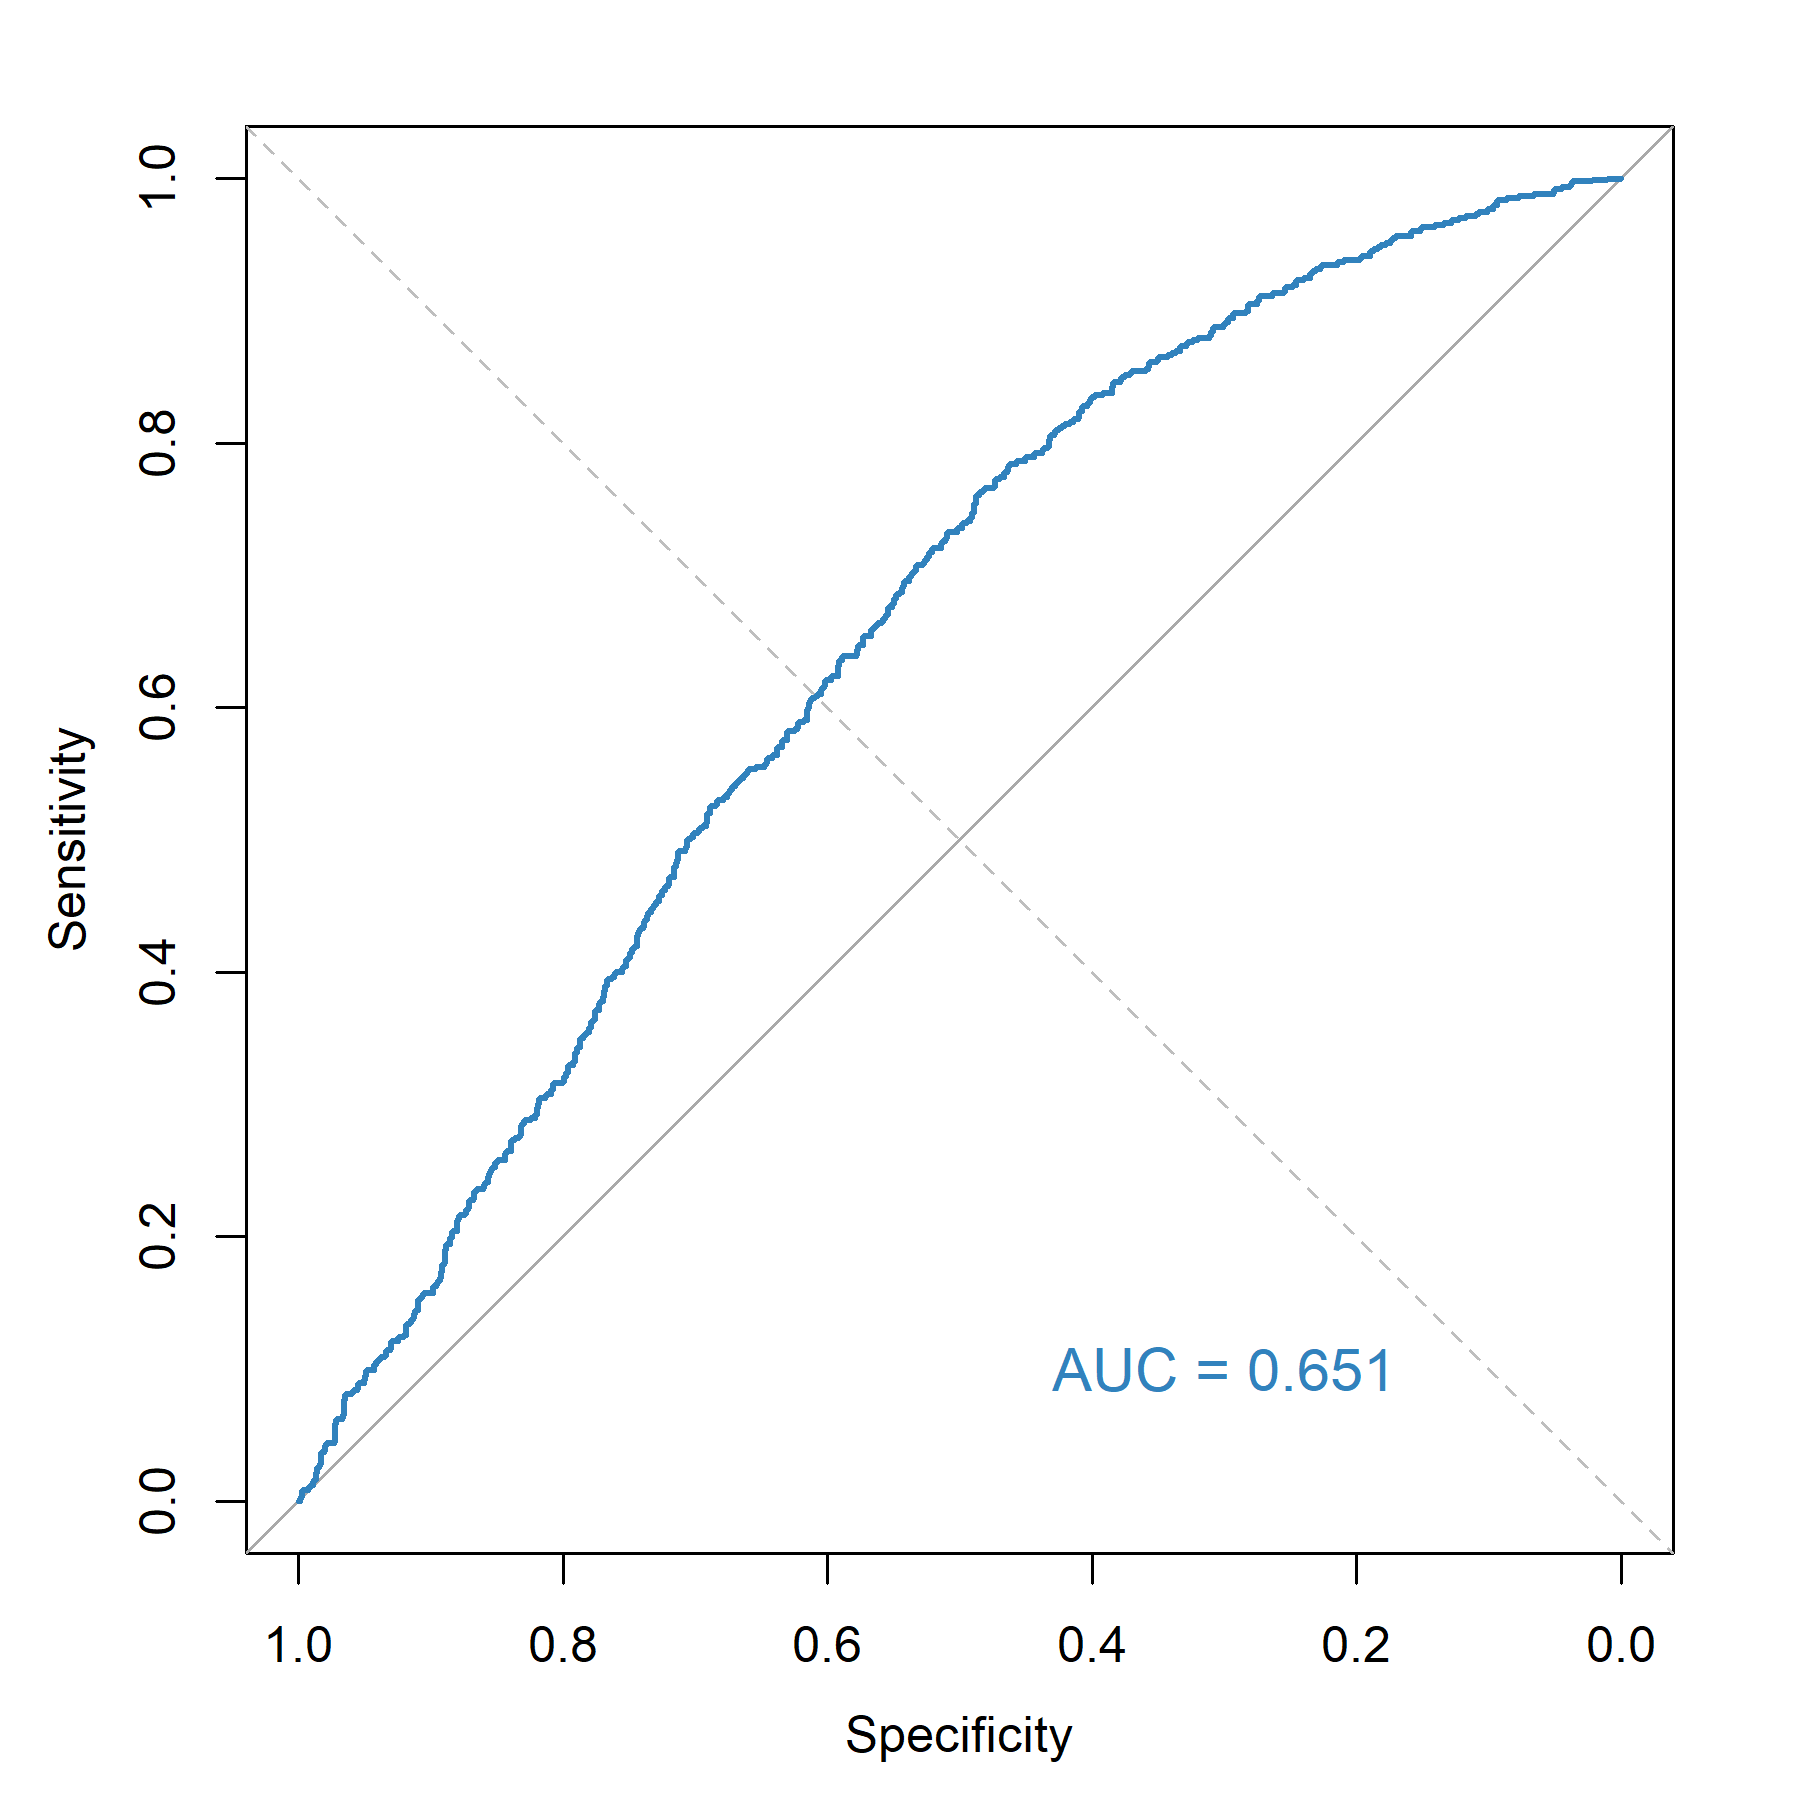
\includegraphics[width=0.50\linewidth]{FIG/12_curva_roc.png}
  \caption{Curva ROC del modelo LGCP (AUC = 0,651). El eje horizontal es la
           tasa de falsos positivos (celdas sin evento clasificadas como de alta
           amenaza) y el eje vertical la tasa de verdaderos positivos (celdas con
           evento correctamente identificadas). La línea diagonal punteada
           representa un clasificador aleatorio (AUC = 0,5).}
  \label{fig:roc}
\end{figure}

% ─────────────────────────────────────────────────────────────
\section{Discusión}
\label{sec:discussion}
% ─────────────────────────────────────────────────────────────

\subsection{Control topohidrológico de la iniciación}

Los coeficientes estimados del modelo LGCP confirman que la topografía es el
principal determinante de la distribución espacial de los movimientos en masa
en el Valle de Aburrá. La pendiente y el TWI exhiben efectos prácticamente
idénticos en magnitud ($\hat{\beta}_1 = 13{,}09$ y $\hat{\beta}_2 = 13{,}00$),
lo que sugiere que los mecanismos de inestabilidad mecánica (pendiente) y los
hidrológicos (saturación) contribuyen de manera comparable a la probabilidad de
iniciación. Este resultado es coherente con el modelo de talud infinito bajo
condiciones saturadas, en el que el factor de seguridad puede expresarse como:
\begin{equation}
  \text{FS} = \frac{c'}{z\,\gamma_s\,\sin\beta\cos\beta}
    + \frac{\tan\phi'}{\tan\beta}
    \left(1 - \frac{\gamma_w}{\gamma_s}\,\frac{h_w}{z}\right),
  \label{eq:fs}
\end{equation}
donde $h_w/z$ es el grado de saturación del suelo, directamente relacionado con
el TWI a través del modelo de balance hídrico de \citet{beven1979}. En este marco,
la reducción de FS $<1$ requiere simultáneamente pendiente alta y saturación
elevada, condición que el LGCP captura a través de los efectos aditivos de ambas
covariables en la log-intensidad.

La magnitud de los coeficientes $(\beta_1, \beta_2 \approx 13)$ puede parecer
excepcionalmente grande, pero esto es consecuencia directa del modelo de proceso
puntual: en la escala de log-intensidad (eventos por metro cuadrado), un
incremento pequeño en las covariables puede producir cambios grandes en la
intensidad porque el rango dinámico de $\lambda(\mathbf{s})$ es enorme
(desde $\approx 10^{-9}$ en zonas planas hasta $\approx 10^{-5}$ en laderas
escarpadas). Los coeficientes deben interpretarse siempre en el contexto del
cambio en intensidad relativa, no como probabilidades absolutas.

El efecto del aspecto ($\hat{\beta}_3 = 5{,}70$), aunque menor, es
estadísticamente robusto y físicamente coherente. Las laderas orientadas hacia
el norte en el Valle de Aburrá reciben menor radiación solar directa,
principalmente durante las horas de la mañana y en los meses de la temporada
de lluvias. Esta menor energía disponible para la evapotranspiración mantiene
mayor contenido de agua en el suelo, prolongando el período de vulnerabilidad
tras los eventos de precipitación. Adicionalmente, las laderas en sombra tienden
a tener coberturas vegetales más densas en las partes altas y pastizales o
tierras degradadas en las partes bajas, con diferente capacidad de anclaje
radicular. Esto explica por qué el aspecto, pese a no ser un factor mecánico
directo, emerge como predictor significativo de la susceptibilidad.

\subsection{Agrupamiento espacial residual: implicaciones geológicas y antrópicas}

El GRF latente con $\hat{\rho} = 5{,}01$ km y $\hat{\sigma}^2 = 2{,}62$ revela
que una fracción sustancial de la variabilidad espacial en la intensidad de
movimientos en masa no queda explicada por la topografía. La desviación estándar
residual $\hat{\sigma} \approx 1{,}62$ en la escala de log-intensidad implica que
en zonas vecinas con topografía idéntica, la intensidad puede variar por un factor
de hasta $e^{2\hat{\sigma}} \approx 26$ debido a factores no topográficos. Este
resultado tiene implicaciones prácticas importantes: los modelos basados únicamente
en atributos del MDE tienen un techo de desempeño discriminativo.

El rango espacial de $\hat{\rho} \approx 5$ km es consistente con la escala de
las principales unidades geológicas del Valle de Aburrá: los afloramientos de
gneis del Complejo Cajamarca, los depósitos aluviales y los coluviones cuaternarios
tienen extensiones típicas del orden de varios kilómetros. La mayor susceptibilidad
de los esquistos y coluviones frente a los gneis frescos, por ejemplo, se
manifesta como un patrón espacial con escala coherente con el rango estimado del
GRF. De forma similar, las zonas de intervención antrópica intensa (urbanización
en ladera, cortes de vía, redes de alcantarillado que aumentan la infiltración
local) exhiben clusters espaciales de actividad de movimientos en masa a escala
kilomètrica, consistente con $\hat{\rho}$.

El campo latente de la Figura~\ref{fig:field} ofrece un mapa operativo del
agrupamiento residual: las zonas con $\xi(\mathbf{s}) > 0$ son prioritarias para
investigación de campo adicional y para la incorporación de variables geológicas
y de uso del suelo en versiones futuras del modelo.

\subsection{Desempeño discriminativo y comparación con la literatura}

El AUC de $0{,}651$ es inferior al de modelos de susceptibilidad que incorporan
geología y uso del suelo, pero es comparable al reportado por \citet{lombardo2019}
para modelos LGCP con predictores exclusivamente topográficos en Sicilia (AUC
$\approx 0{,}63$--$0{,}67$). La principal limitación del desempeño discriminativo
en el presente estudio es la ausencia de variables que controlan la susceptibilidad
litológica y la intervención antrópica. En el Valle de Aburrá, los movimientos
en masa en suelos derivados de coluviones y depósitos de vertiente tienen una
susceptibilidad significativamente mayor que los desarrollados sobre el macizo
rocoso, diferencia que no puede ser capturada por la topografía sola.

Cabe resaltar que el AUC de $0{,}651$ se evalúa a una escala de \SI{500}{m}
(tamaño de celda hexagonal), que es la escala a la que el modelo aporta información
discriminativa. A escalas más gruesas (e.g., cuadrantes de $1\,\text{km}^2$),
el AUC sería previsiblemente mayor, dado que la suavización espacial reduce la
varianza del conteo observado y aumenta la correlación con el modelo. En contraste,
a la escala del punto (evento individual), el AUC reflejaría la estocasticidad
intrínseca de los movimientos en masa ante condiciones de lluvia específicas,
lo que daría valores más bajos. La escala de evaluación es, por tanto, una
decisión de diseño que debe ajustarse a la resolución operativa del sistema de
gestión del riesgo.

\subsection{Confusión espacial y robustez de los coeficientes}

Una preocupación inherente a los modelos con GRF y covariables espaciales es la
confusión espacial \citep{hanks2015}: si las covariables varían espacialmente a
la misma escala que el GRF, este puede absorber parte de los efectos de las
covariables, sesgando los coeficientes hacia cero. En experimentos diagnósticos
preliminares, modelos sin GRF arrojaron $\hat{\beta}_1 \approx 120$--$182$,
valores que se redujeron a $\approx 13$ al incorporar el GRF con priors informativas.
Este fenómeno indica que el GRF absorbe una parte del efecto de la pendiente que
opera a escala geológica (la misma escala que el rango del GRF). Sin embargo,
los coeficientes con GRF son más conservadores y representan el efecto de la
pendiente \textit{condicionado} sobre el agrupamiento residual, lo que los hace
más robustos para predicción en áreas con distinto sustrato geológico.

\subsection{Extensiones futuras}

Los resultados sugieren varias extensiones prioritarias del modelo. La más inmediata
es la incorporación de variables geológicas (unidad litológica, espesor del regolito)
y de cobertura del suelo (bosque nativo, pastizal, área urbanizada), que se
espera reduzca la varianza del GRF residual y aumente el AUC por encima de
$0{,}70$--$0{,}75$. Una segunda extensión es la modelación espacio-temporal,
posible cuando el inventario incluye fechas de ocurrencia y datos de precipitación:
el LGCP puede extenderse a un proceso de Cox espacio-temporal con intensidad
$\lambda(\mathbf{s},t)$ \citep{lombardo2020}, permitiendo modelar la variación
estacional de la amenaza y la correlación entre eventos disparados por la misma
tormenta. Una tercera línea es la incorporación de incertidumbre en el inventario
mismo, dado que los registros históricos son incompletos para áreas de difícil
acceso; marcos de detección-covariable pueden integrarse en el LGCP para modelar
el sesgo de observación espacialmente variable \citep{diggle2013lgcp}.

% ─────────────────────────────────────────────────────────────
\section{Conclusiones}
\label{sec:conclusions}
% ─────────────────────────────────────────────────────────────

\textit{[Por completar por el autor.]}

% ─────────────────────────────────────────────────────────────
\section*{Agradecimientos}
% ─────────────────────────────────────────────────────────────

\textit{[Por completar.]}

% ─────────────────────────────────────────────────────────────
\section*{Disponibilidad de datos}
% ─────────────────────────────────────────────────────────────

El inventario de movimientos en masa y los rasters topográficos están disponibles
bajo solicitud razonable al autor para correspondencia. El código R se proporciona
como material suplementario.

% ─────────────────────────────────────────────────────────────
\bibliographystyle{abbrvnat}
\bibliography{referencias}
% ─────────────────────────────────────────────────────────────

\end{document}
